%%%%%%%%%%%%%%%%%%%%%%%%%%%%%%%%%%% ESTADO DEL ARTE / STATE OF THE ART CHAPTER %%%%%%%%%%%%%%%%%%%%%%%%%%%%%%%%%

\chapter{Related work}
\label{cha:related-work}

This chapter overviews the state of the art in three key areas of Computer Vision relevant to this master thesis: semantic segmentation, generative models, and explainability. This review aims to establish a comprehensive understanding of the methods explored in this thesis, as well as to contextualize the motivation of synthetic data generation to develop semantic segmentation methods.

The chapter is divided into three sections, each focusing on the aforementioned areas. We start by exploring the challenges of semantic segmentation and the various approaches taken to overcome the lack of annotated data. Next, we delve into the literature on generative models, with a specific emphasis on the recent Stable Diffusion architecture that is used to generate synthetic images in this work. Finally, we discuss the issue of explainability in Computer Vision, concentrating notably on attention-based methodologies. We specifically examine the ongoing research that employs attention maps for achieving explainability in Latent Diffusion Models. These maps serve as a pivotal approach in text-to-image models, attributing the influence of input prompts on the images generated.


%%%%%%%%%%%%%%%%%%%%%%%%%%%%%%%%%%%%%%%%%%%%%%%%%%%%%%%%%%%%%%%%%%%%%%%%%%%%
%%%%%%%%%%%%%%%%%%%%%%%%%  SEMANTIC SEGMENTATION   %%%%%%%%%%%%%%%%%%%%%%%%%
%%%%%%%%%%%%%%%%%%%%%%%%%%%%%%%%%%%%%%%%%%%%%%%%%%%%%%%%%%%%%%%%%%%%%%%%%%%%

\section{Semantic Segmentation}

Semantic segmentation is a Computer Vision task that aims to assign a semantic label to each pixel of an input image. More formally, the objective is to learn an injective function that maps an image to its corresponding segmentation map, as the one illustrated in Figure \ref{fig:semantic-segmentation-example}.

The task is closely related to other Computer Vision tasks, such as depth estimation, which estimates the depth of each pixel in an image, or lane detection, which predicts the geometry of a road from the perspective of a vehicle. In the domain of urban scenes, solutions to these problems are core components for the development of applications in autonomous driving \cite{Grigorescu2019ASO}. The accuracy and robustness of algorithms for these tasks are critical for developing safe and reliable autonomous vehicles.

Despite significant progress in recent years, semantic segmentation remains a challenging task due to the high variability of natural scenes, as well as the limited availability of annotated data. To address the lack of annotated data, researchers have explored various approaches, such as transfer learning, domain adaptation, and synthetic data generation. In the following subsections, we discuss these approaches in detail.


\begin{figure}
    \centering
    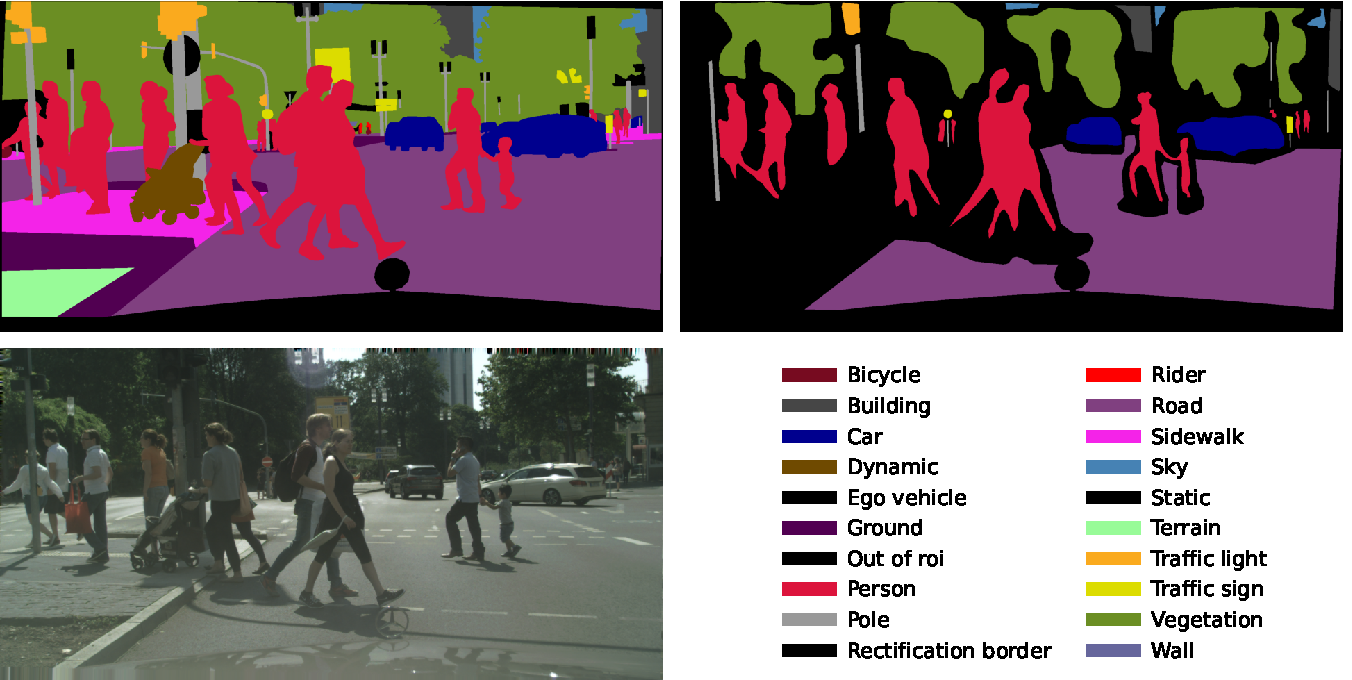
\includegraphics[width=1\columnwidth]{img/2-related-work/1-example-annotation.pdf}
    \caption[Example of semantic segmentation annotations]{Example of an urban scene with semantic segmentation annotations from the Cityscapes Dataset \cite{Cityscapes}. Top-left: Fine-grained ground-truth annotation. Top-right: coarse annotation. Bottom-left: image. Bottom-right: semantic classes.}
    \label{fig:semantic-segmentation-example}
\end{figure}
    

%%%%%% Subsection: architectures


\subsection{Architectures}


Deep convolutional neural networks have emerged as the leading approach to address semantic segmentation \cite{Chai2021}. Unlike other tasks such as classification, where the output of the models is a vector with one score per class, semantic segmentation requires the prediction of a score for each pixel of the input image and its corresponding semantic class, making it a computationally demanding operation. 

Although researchers have proposed successful architectures that process images while maintaining the spatial dimension internally in all layers \cite{Sun2019HighResolutionRF}, the use of such architectures comes with a high computational cost.
For this reason, the most common architectures downsample the images with convolutional layers to reduce computational requirements and upsample the compact representation to produce an output of the same size as the input. This takes advantage of spatial locality, making the process more computationally efficient \cite{SemanticSegmentationSurvey}.


One of the earliest architectures that proposes the aforementioned approach is the Fully Convolutional Network (FCN) \cite{FCN}. FCN uses several convolutional layers to reduce the spatial dimension of the input image while increasing the number of channels to maintain local semantic information. A final pixel-wise layer is used to generate a detailed segmentation, as illustrated in Figure \ref{fig:fcn}.


\begin{figure}
    \centering
    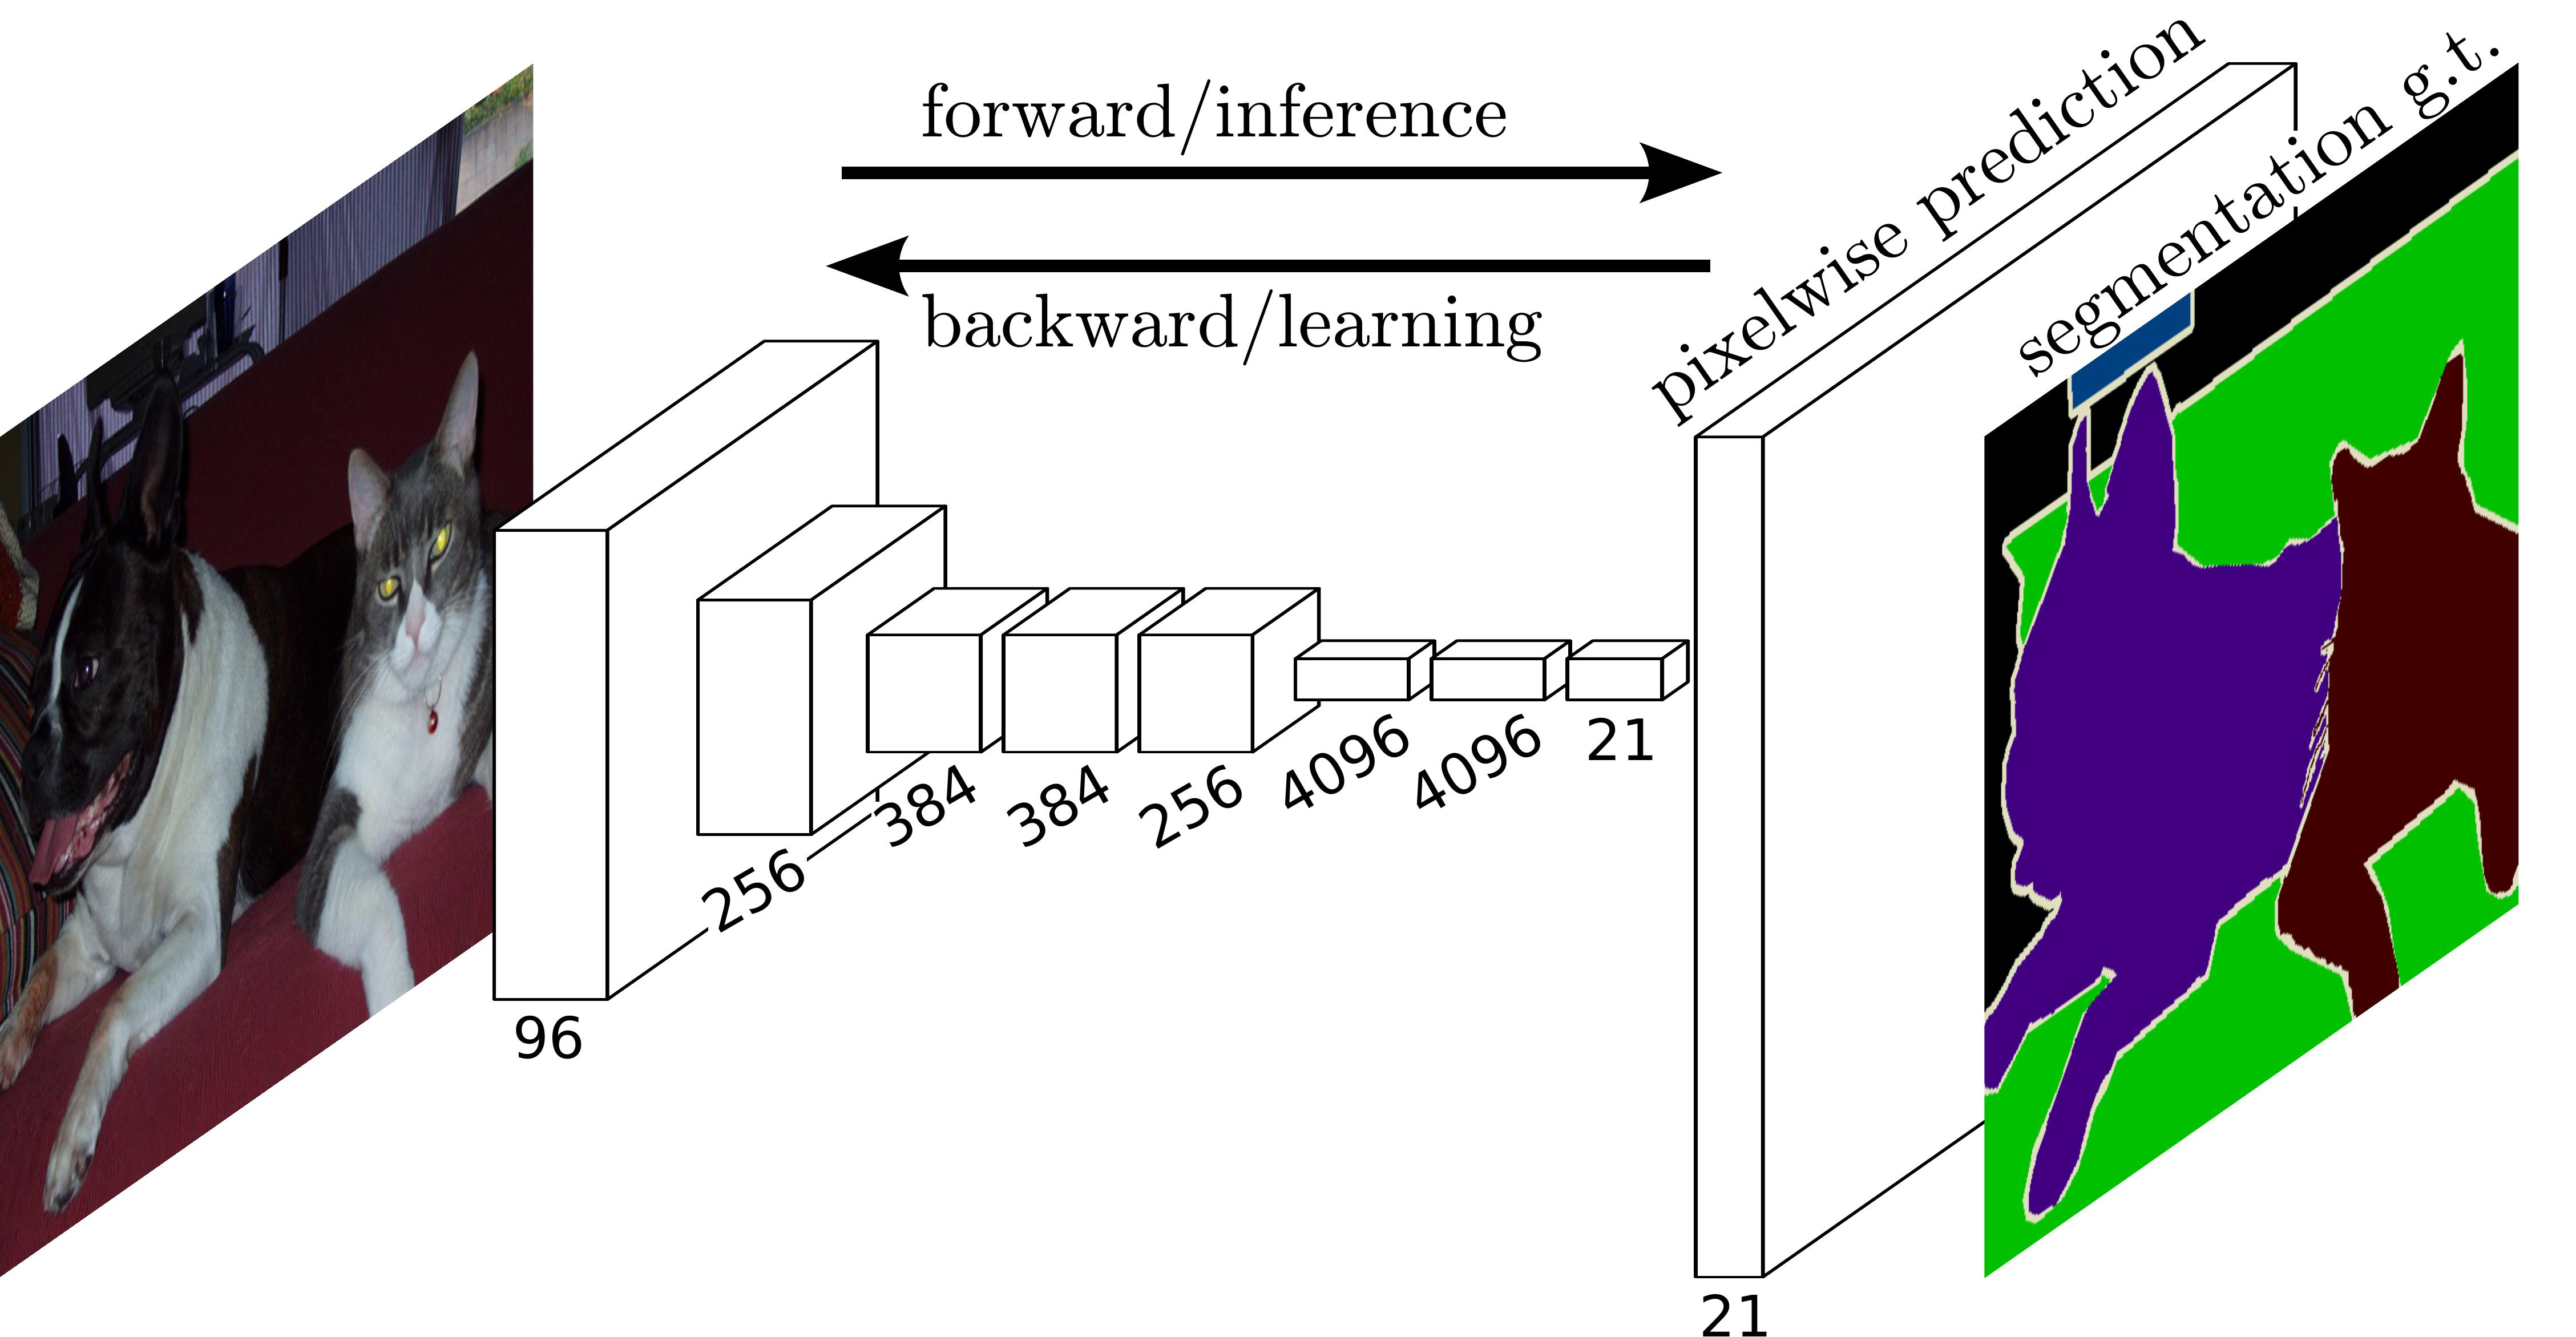
\includegraphics[width=0.7\columnwidth]{img/2-related-work/design-fcn.jpeg}
    \caption[Fully convolutional network n (FCN)]{Fully convolutional network for semantic segmentation \cite{FCN}}
    \label{fig:fcn}
\end{figure}

To prevent the potential loss of spatial information due to the downsampling layers, researchers proposed the U-NET architecture \cite{UNET}, a symmetric encoder-decoder design (shown in Figure \ref{fig:unet}) that incorporates connections between the downsampling and upsampling stages. These connections merge the semantic information from the higher layers with the spatial information from the lower layers obtaining fine-grained predictions.

Many contemporary semantic segmentation architectures are being proposed in this direction, aiming to compactly encode semantic information while minimizing spatial information loss. As an example, two popular approaches are the use of atrous convolutions and multi-resolution features. 
Atrous convolutions \cite{DeeplabV3}, also known as dilated convolutions, increase the receptive field by introducing gaps between kernel elements, resulting in the efficient processing of high-resolution images without increasing the number of parameters. On the other hand, multi-resolution features, used in HRNet \cite{HRNET}, involves using convolutions of different sizes in parallel to extract information at multiple levels of resolution and combine it for a more robust representation. This strategy allows the use of features with complementary information, improving accuracy and enabling fine-grained predictions. 

Since these models are complex and require large amounts of data, training strategies such as curriculum learning \cite{Zhang2017}, knowledge distillation \cite{Tung2019SimilarityPreservingKD}, and adversarial losses \cite{Tsai_adaptseg_2018} are commonly used to improve their performance. For this reason, much of the research efforts are based on exploring new training strategies and creating datasets with increased variability, particularly in domains such as urban scenes. In the following subsection, we introduce some of the most widely used datasets and benchmarks for training and compare the performance of these models.

\begin{figure}
    \centering
    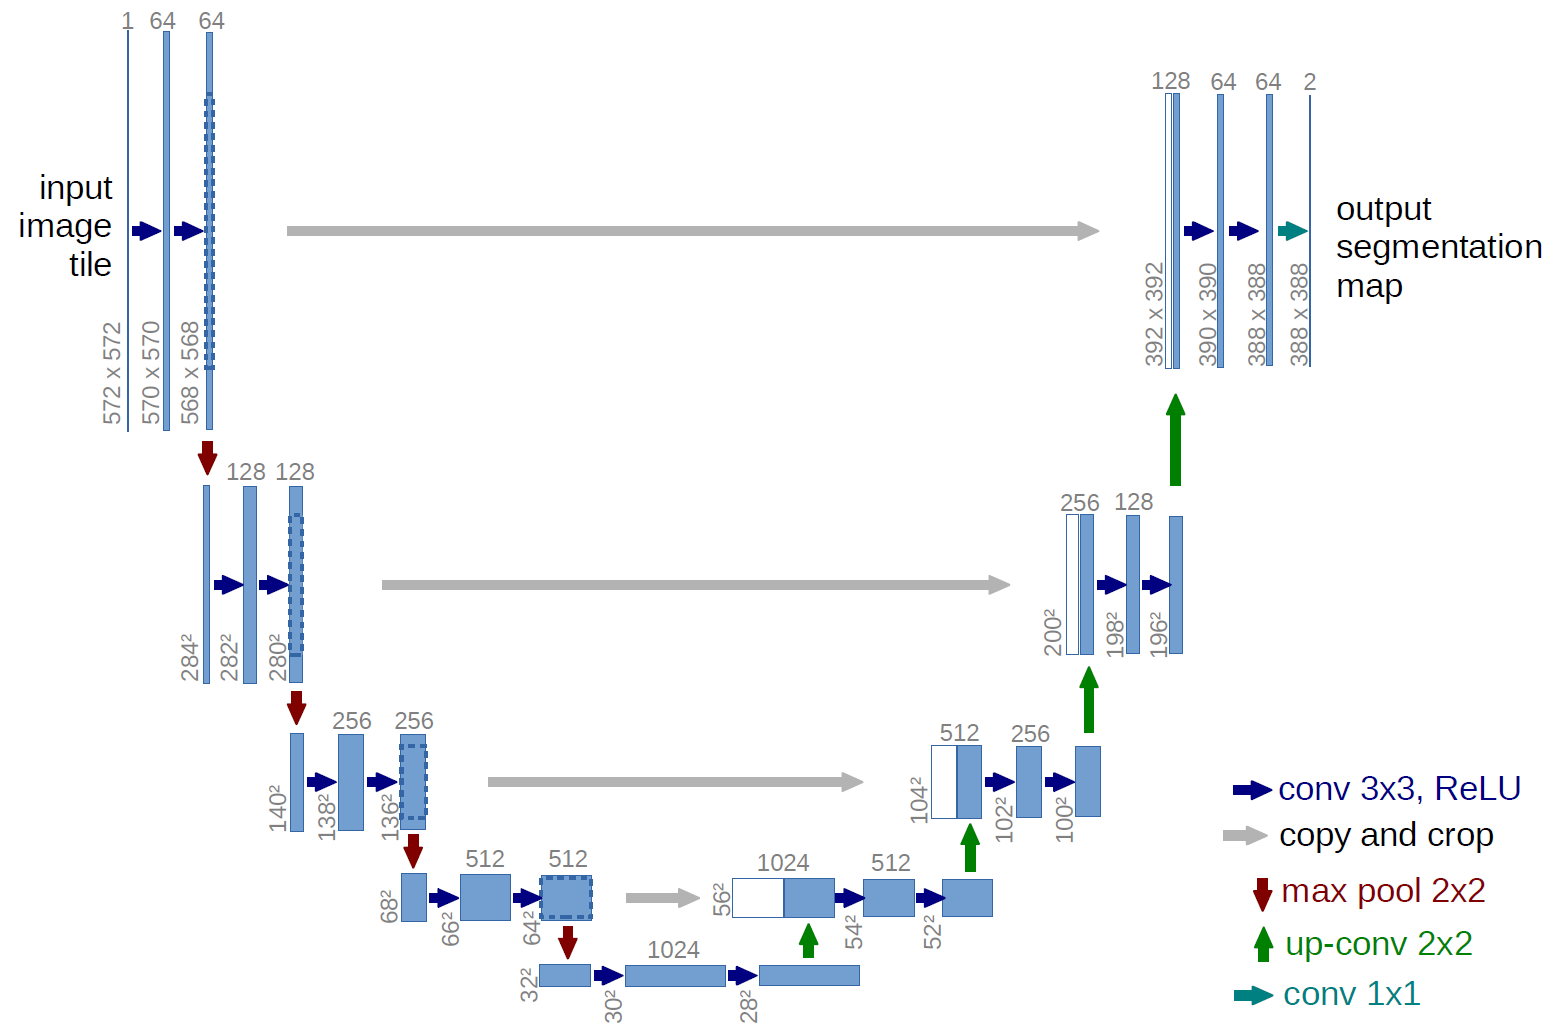
\includegraphics[width=0.75\columnwidth]{img/2-related-work/u-net-architecture.png}
    \caption[U-NET architecture]{U-NET architecture. Source \cite{UNET}.}
    \label{fig:unet}
\end{figure}

\subsection{Datasets and benchmarks}

%% Example of real datasets
\begin{figure}
\centering
  \begin{subfigure}[b]{0.49\columnwidth}
    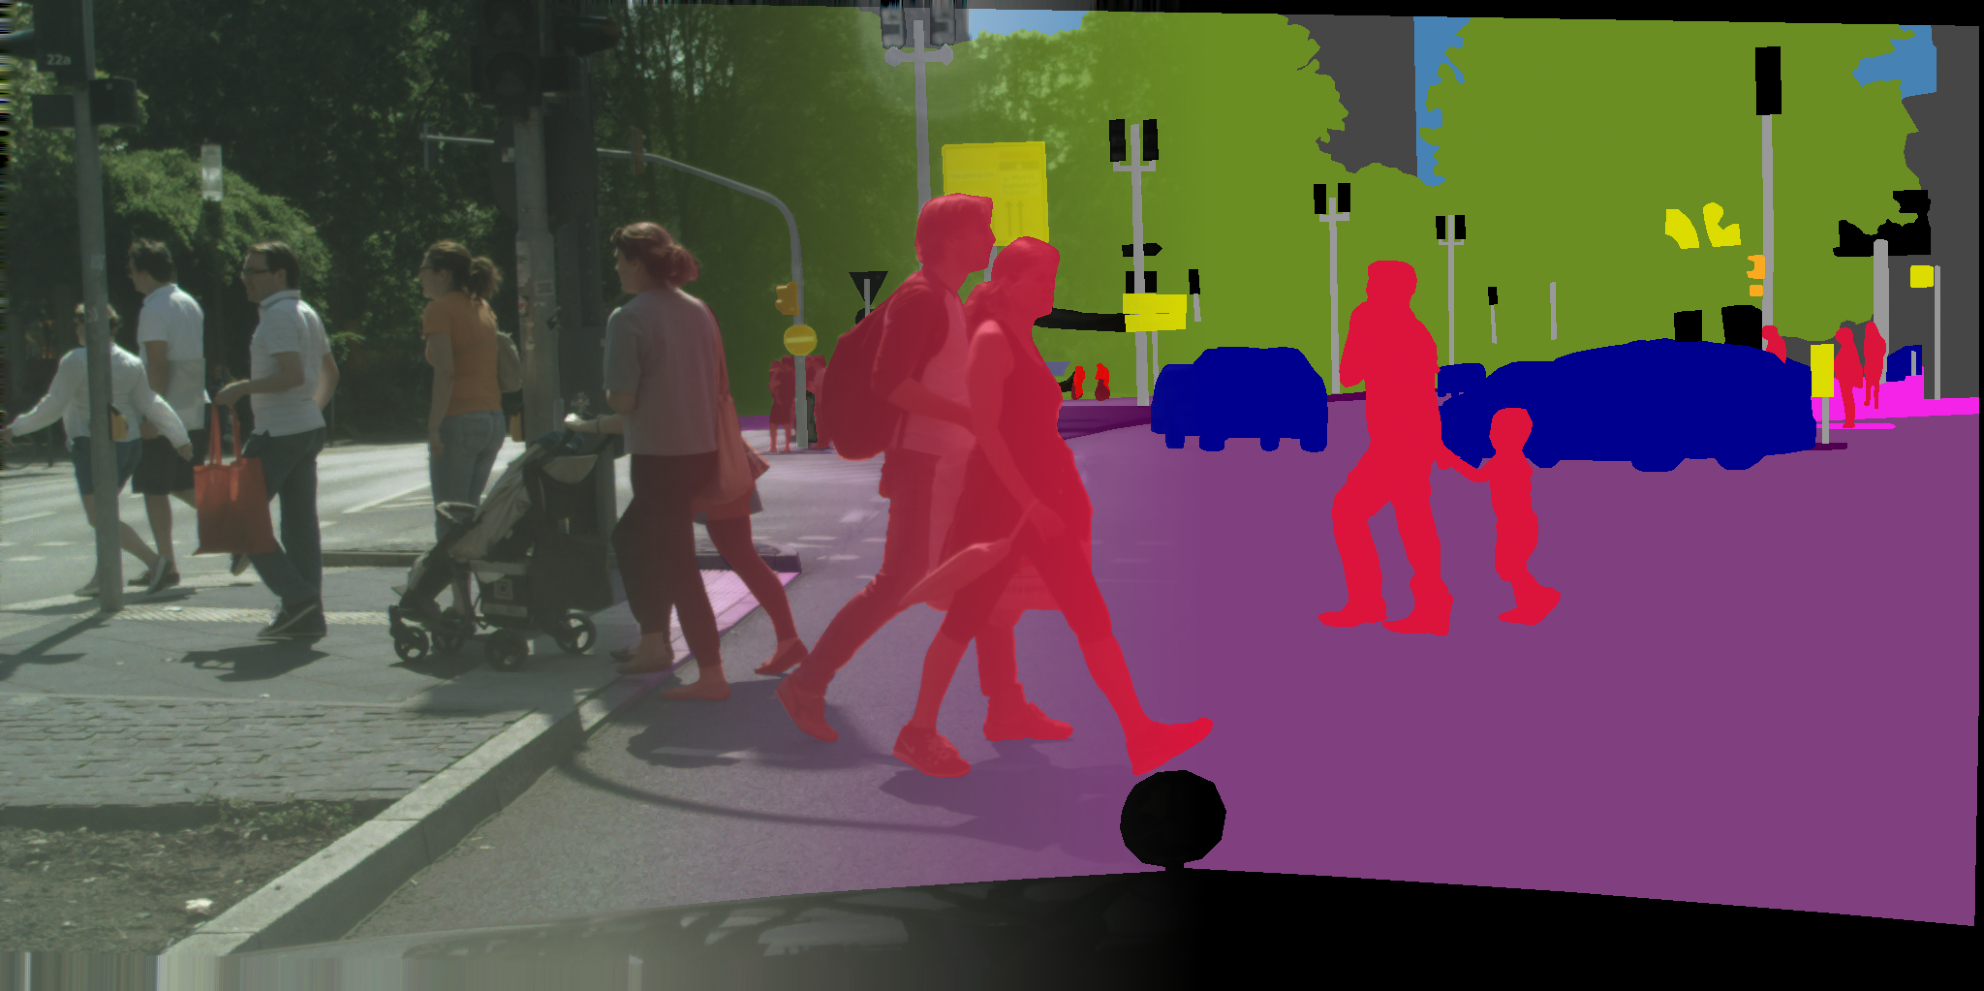
\includegraphics[width=\columnwidth]{img/2-related-work/cityscapes_semantic_segmentation_overlay.png}
    \caption{Cityscapes \cite{Cityscapes}}
    \label{fig:example-city}
  \end{subfigure}
  %
  \begin{subfigure}[b]{0.49\columnwidth}
    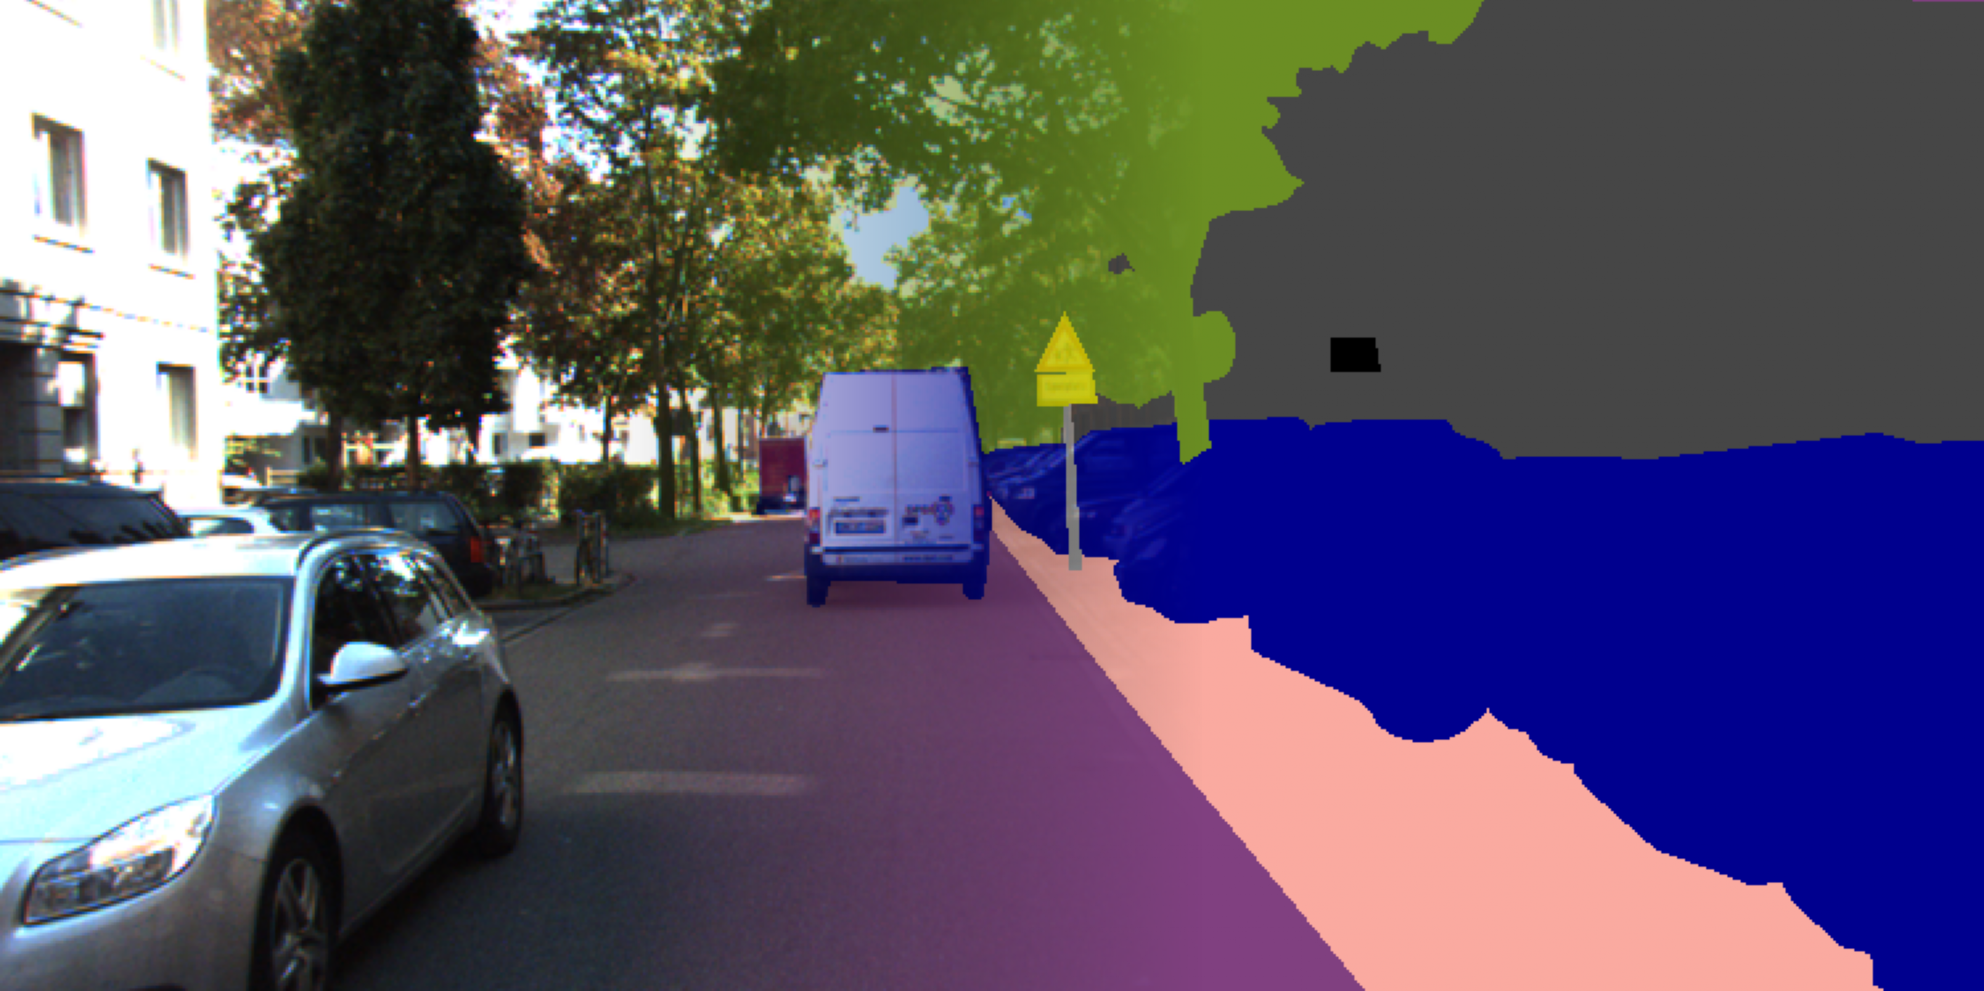
\includegraphics[width=\columnwidth]{img/2-related-work/kitti_semantic_segmentation_overlay.png}
    \caption{KITTI \cite{kitty}}
    \label{fig:example-kitti}
  \end{subfigure}

  \begin{subfigure}{0.49\columnwidth}
    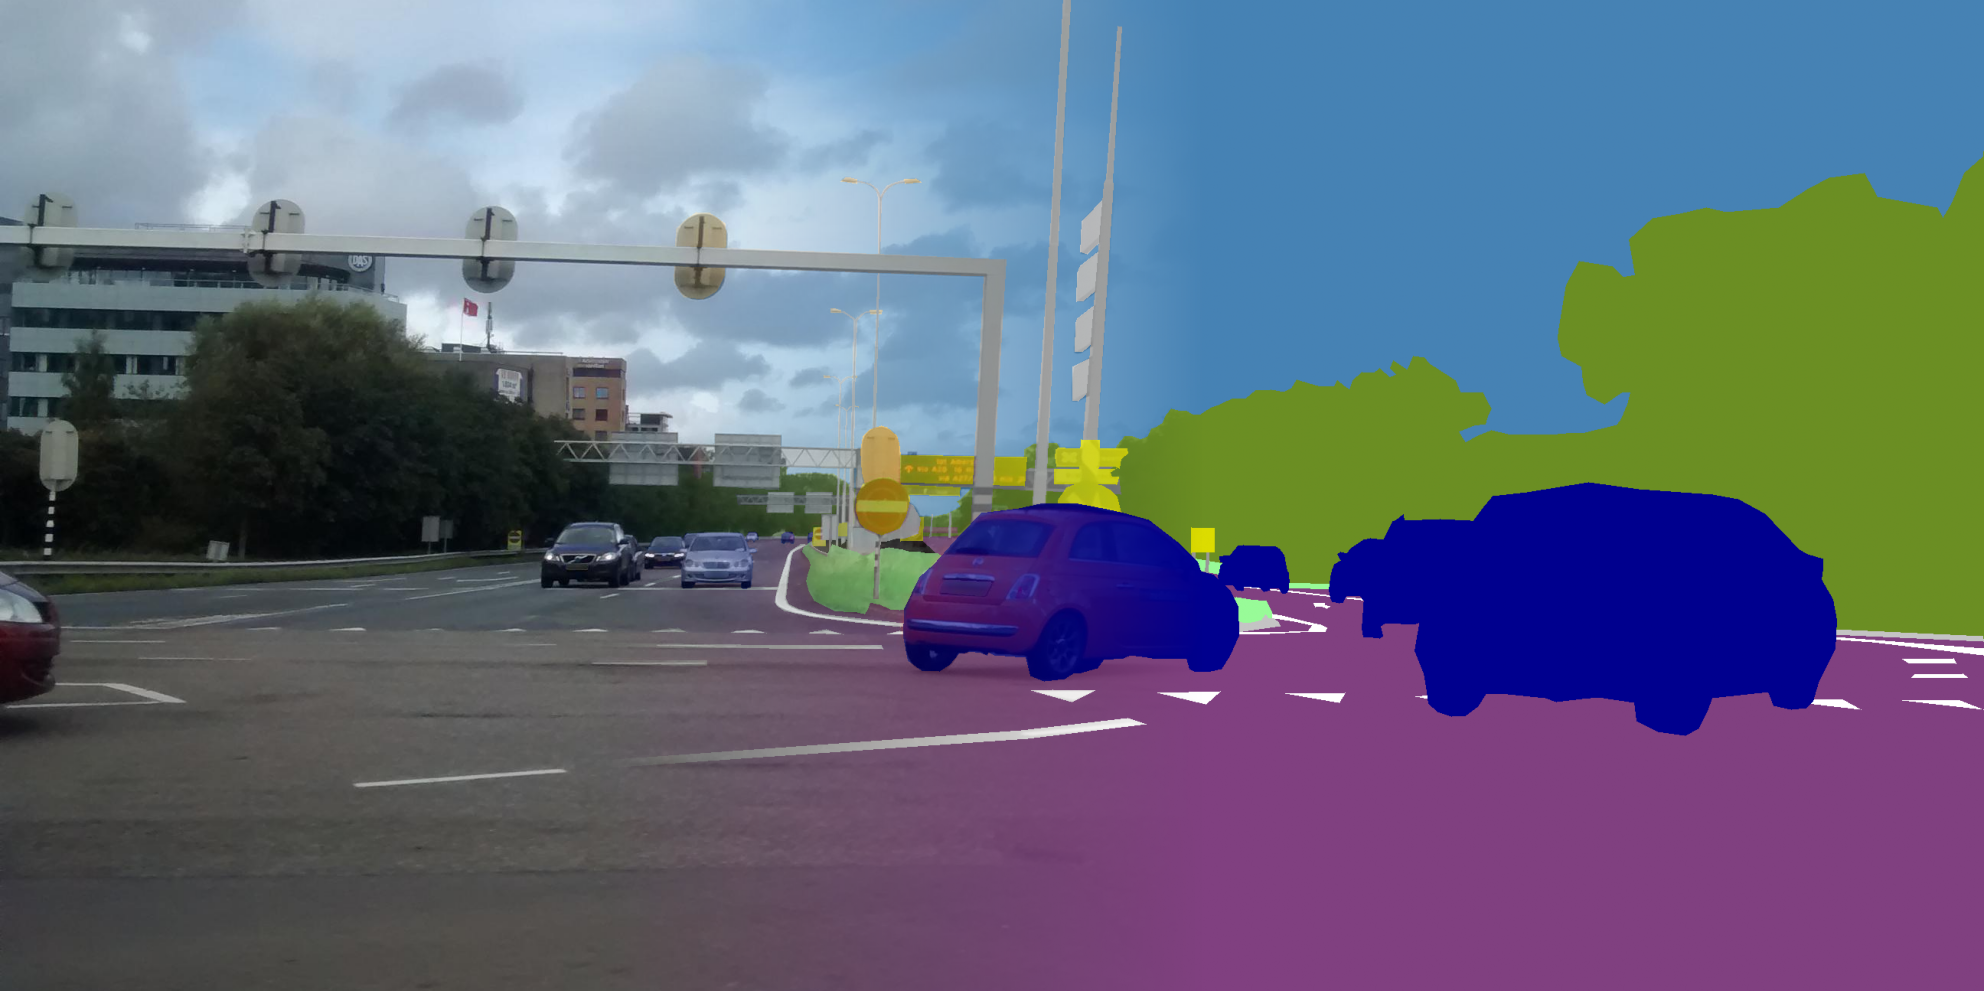
\includegraphics[width=\columnwidth]{img/2-related-work/mapilliary_semantic_segmentation_overlay.png}
    \caption{Mapillary Vistas \cite{mapilliary}}
    \label{fig:example-dbb100k}
  \end{subfigure}
  %
  \begin{subfigure}[b]{0.49\columnwidth}
    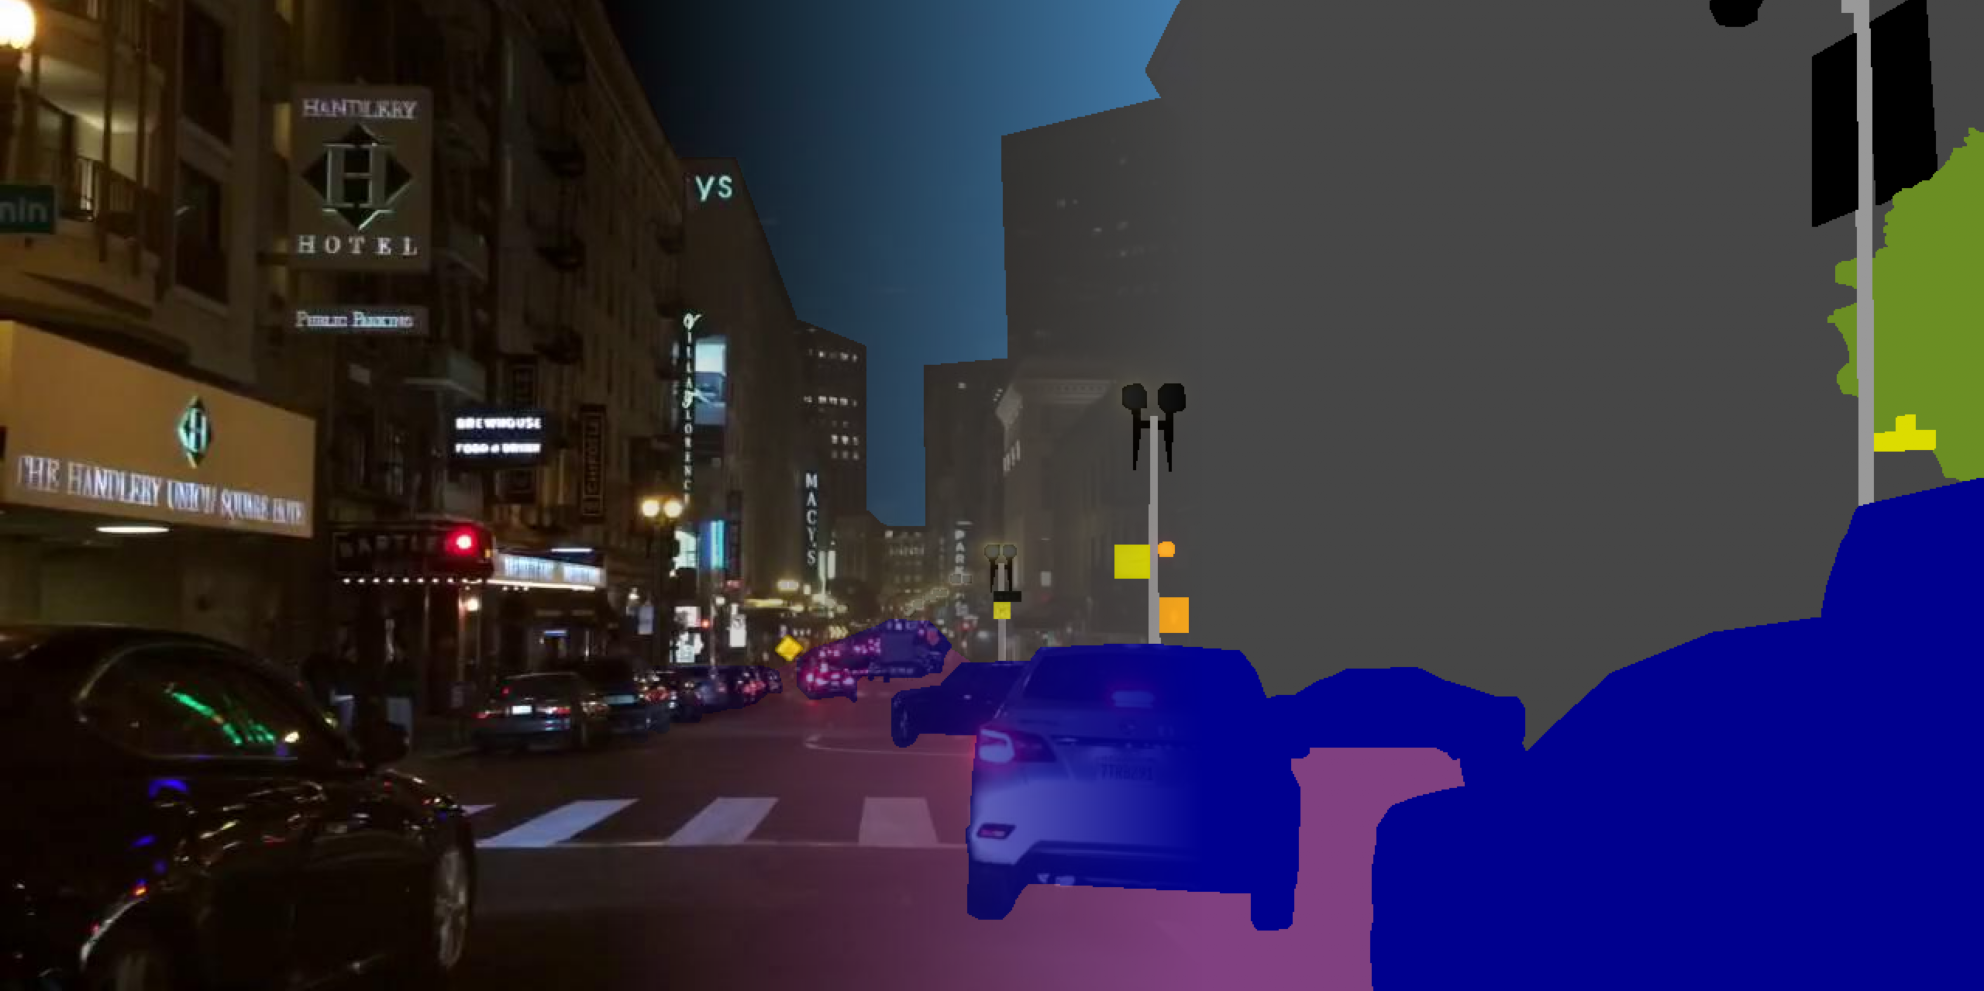
\includegraphics[width=\columnwidth]{img/2-related-work/dbb100k_semantic_segmentation_overlay.png}
    \caption{Berkeley Deepdrive Dataset \cite{BDD100K}}
    \label{fig:example-mapilliary}
  \end{subfigure}

  \caption[Visual examples of real datasets for urban scenes]{Visual examples of real datasets for urban scenes}
    \label{fig:real-datasets-examples}

\end{figure}

%Semantic segmentation is a challenging task that requires complex deep learning models, massive amounts of data, and specialized training strategies to achieve competitive performances. 
One of the main factors contributing to the success of semantic segmentation models is the availability of large datasets with high-quality annotations for training and evaluation. To address this issue, the research community has created several public datasets and benchmarks to train these models and unify comparisons. In this section, we review the most commonly used real datasets for semantic segmentation of urban scenes. 

Urban scenes datasets are composed of images taken from cameras on moving vehicles or captured by drones, and commonly they show the urban environment from the driver's point of view. These images are annotated with pixel-level labels with different semantic categories, such as roads, buildings, pedestrians, and vehicles. The annotations are used as ground truth segmentation maps to train and evaluate semantic segmentation models. Some of the most widely used datasets in this area, illustrated in Figure \ref{fig:real-datasets-examples}, are Cityscapes \cite{Cityscapes}, KITTI \cite{kitty}, Mapillary \cite{mapilliary}, and BDD100K \cite{BDD100K}.

Cityscapes \cite{Cityscapes} contains high-quality images of street scenes from 50 different cities across Europe, with pixel-level annotations of 30 different semantic classes. KITTI \cite{kitty} contains images of urban scenes captured by a camera mounted on a moving vehicle and annotated with semantic labels. Mapillary \cite{mapilliary} is a crowd-sourced dataset that contains images taken from street-level perspectives by a large community of users with global coverage. BDD100K \cite{BDD100K} contains diverse and challenging images with different weather conditions in urban and suburban areas. Table \ref{tab:real-datasets} contains information of these and other of the most widely used datasets of urban scenes.

\begin{table}
    \centering
    \begin{tabular}{|c|c|c|c|}
         \hline 
         Dataset & Geographic coverage & Classes & Public images \\
         \hline 
          Cityscapes \cite{Cityscapes} & 50 cities (Germany) & 30 & 
          5,000 (+20,000)  \\ 
          KITTI \cite{kitty}  & 1 city (Germany) & 30 & 200 \\
          Mapillary Vistas \cite{mapilliary}  & Global coverage & 124 & 20,000 \\
          Berkeley DeepDrive \cite{BDD100K}  & 4 cities (USA) & 40 & 10,000 \\
          Wilddash2 \cite{wildash2}  & Global coverage & 30 & 4,256 \\
          Apollo Scape \cite{wang2019apolloscape}  & 4 regions in China & 25  & 146,997 \\
          India Driving Dataset \cite{Varma_2019} & 182 scenes (India)  & 34 & 10,000 \\
          Audi A2D2 \cite{Geyer2020A2D2AA}  & South of Germany & 38 & 41,277 \\
           \hline
    \end{tabular}
    \caption[Summary of widely used real datasets]{Summary of widely used datasets in semantic segmentation of urban scenes}
    \label{tab:real-datasets}
\end{table}

As a way to increase the variability and the number of annotated images, some datasets provide low-quality annotations that can be used for pre-training. For example, Cityscapes provides 20,000 extra coarse annotations (as shown in Figure \ref{fig:semantic-segmentation-example}). However, due to the high cost of manually annotating images with high detail \cite{Lin_2019_ICCV}, these datasets consist of only a few thousand images. Despite the effort to create more diverse and high-quality datasets, a still unsolved problem is the high bias between them. Models trained on a dataset do not generalize correctly to other ones due to differences in image quality, lighting conditions, and annotation criteria \cite{mapilliary}. This issue is known as domain shift and is one of the main challenges in semantic segmentation research.

To enable the comparison of different models under the same conditions, it is necessary to define a set of evaluation metrics. To address this problem, the research community has created benchmarks associated with each of the main datasets to evaluate models under the same conditions. The most common metric for semantic segmentation is Intersection over Union (IoU), which measures the overlap between the predicted and ground truth segmentation maps. Although other metrics, such as precision and recall, are also used to evaluate model performance, and the choice of new metrics is still an open discussion in the research community \cite{metrics1, Zhang2021RethinkingSS, Cho2021WeightedIO}.




\subsection{Synthetic data}




%\begin{table}
%    \centering
%    \begin{tabular}{|c|c|c|c|}
%         \hline 
%         Dataset & Year & Engine & Notes \\
%         \hline 
%          TORCS & - & - & - \\
%          Virtual KITTI \cite{kitty} & - & - & - \\
%          GTAVision \cite{gtav} & - & - & - \\
%          SYNTHIA \cite{SYNTHIA} & - & - & - \\
%          VIPER & - & - & - \\
%          CARLA \cite{CarlaSimulator} & - & - & - \\
%          AADS & - & - & - \\
%          PreSIL & - & - & - \\
%          MSS & - & - & - \\
%           \hline
%    \end{tabular}
%    \caption[Summary common used synthetic datasets]{Summary of widely used synthetic datasets in semantic segmentation. \emph{NOTA. Citar a Rober, MTAP.}}
%    \label{tab:synthetic-datasets}
%\end{table}


Since the first attempts to develop autonomous driving systems, a major challenge has been the availability of datasets that can capture the variability of driving environments \cite{pomerleau:alvinn}. To address this issue, researchers have employed synthetic data generated by simulators to increase this variability.

In recent years, simulators based on game engines, such as Unity \cite{kitty, SYNTHIA} or GTA V \cite{gtav}, have become popular. Simulators allow the extraction of complete information from the environment, including semantic classes, 3D boxes, multiple perspectives, or depth maps in a pixel-accurate way, as in the examples illustrated in Figure \ref{fig:synthetic-datasets-examples}. 
%Table \ref{tab:synthetic-datasets} provides an overview of widely used synthetic datasets in autonomous driving research.
Other techniques, such as the use of Generative Adversarial Networks \cite{NIPS2014_5ca3e9b1}, have also been employed to increase the amount of data and variability from pre-existing datasets. These methods are typically employed to alter weather or light conditions of scenes, or even to introduce new elements into images.

However, training or pre-training on synthetic data presents challenges due to domain adaptation problems. The domain adaptation problems arise because of the difference in image distributions between synthetic data used for training models and real-world images. Due to this difference, systems lose efficiency when deployed in real-life situations. To mitigate this issue, two primary strategies are used: input and output adaptation.

Input adaptation involves adjusting the synthetic images used during the training step to make them more photorealistic. This can be achieved by using increasingly realistic simulators or by employing generative models to adapt the style of simulator images to make them more photorealistic. However, there is no general consensus on whether photorealism is a necessary aspect that can be solved by increasing the variability in the datasets.

Output adaptation involves incorporating strategies during the training of semantic segmentation models to increase their generalization and reduce the impact of the difference between synthetic and real distributions. This group of strategies includes the use of transfer learning, curriculum learning \cite{Zhang2017}, knowledge distillation \cite{Tung2019SimilarityPreservingKD}, or adversarial losses \cite{Tsai_adaptseg_2018}.

In conclusion, the generation of scenarios capable of including as much variability as possible is fundamental for the development of semantic segmentation systems. Synthetic datasets can include environmental situations that are difficult to simulate and can reduce the need for large real-world datasets, which is crucial for the development of more robust autonomous driving systems. For these reasons, both the scientific community and the industry are putting great efforts into developing new methods for the creation of synthetic data and techniques to reduce the problems of domain shift and domain adaptation.


%% Example of real datasets
\begin{figure}
\centering
  \begin{subfigure}[b]{0.49\columnwidth}
    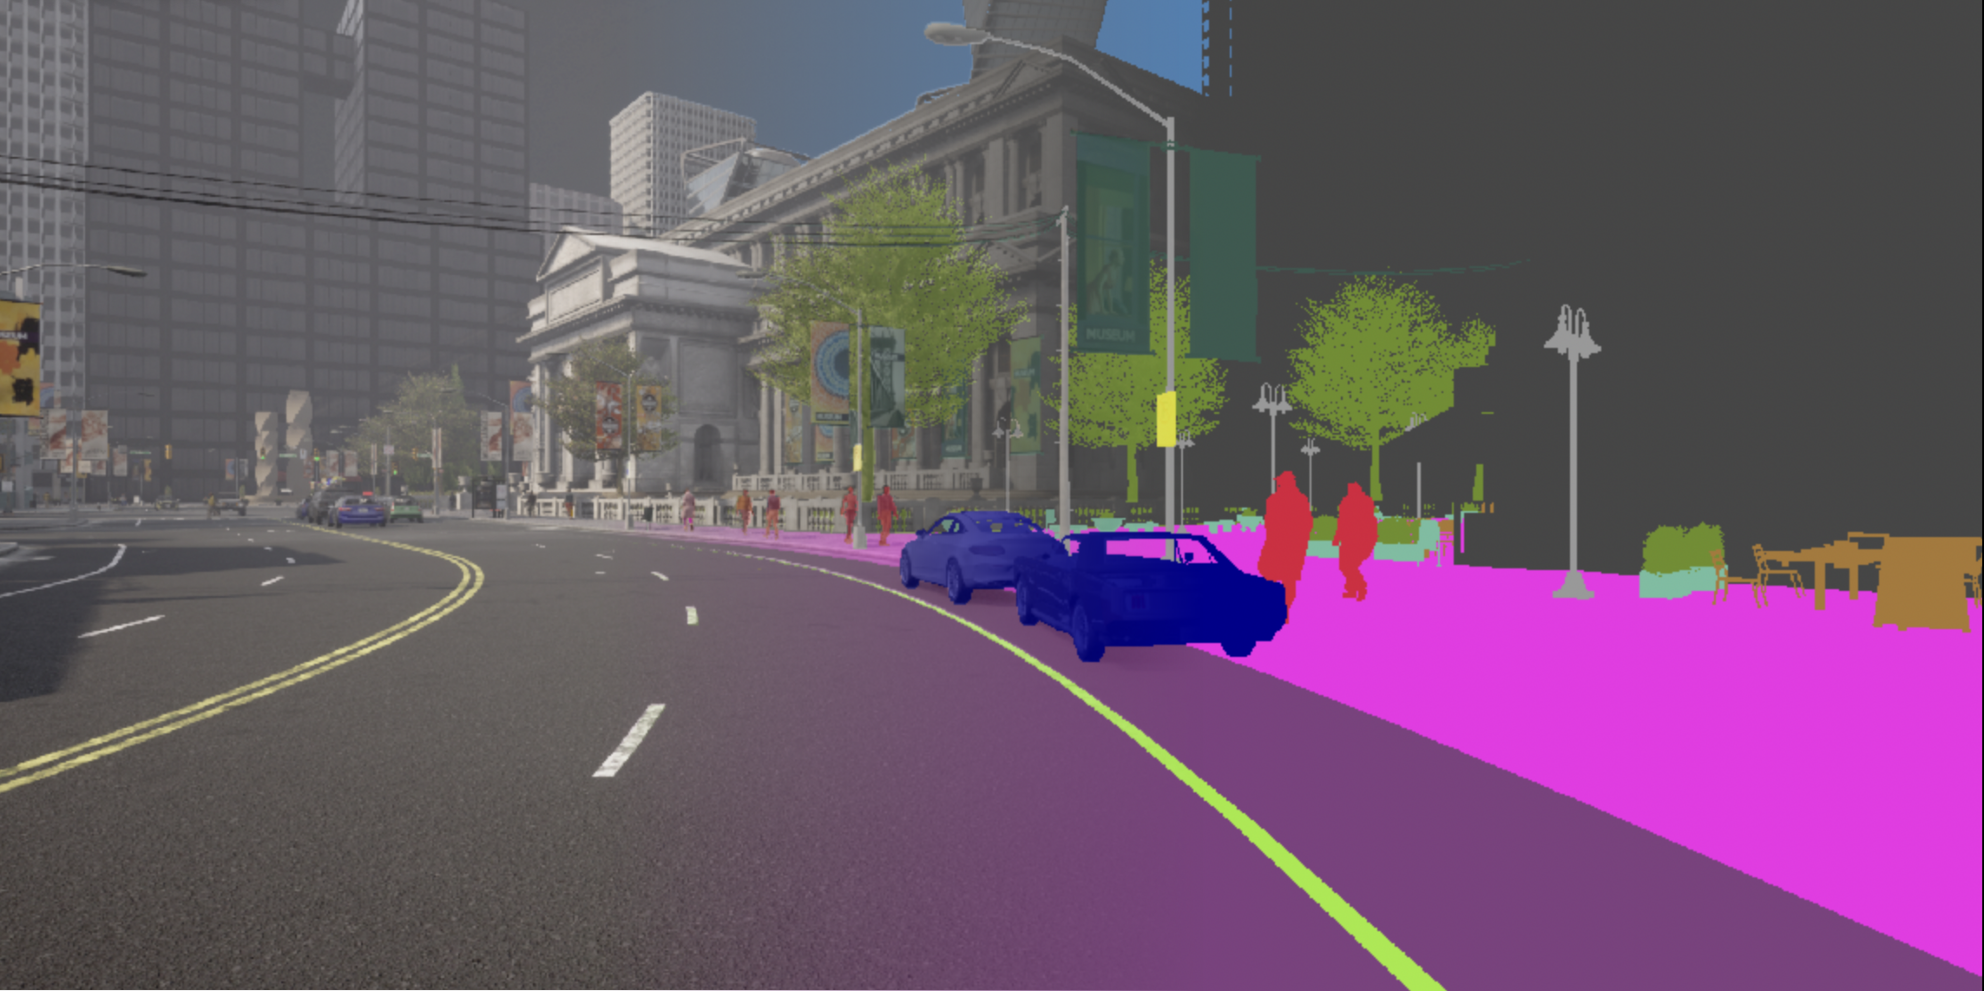
\includegraphics[width=\columnwidth]{img/2-related-work/carla_semantic_segmentation_overlay.png}
    \caption{Carla Simulator \cite{CarlaSimulator}}
    \label{fig:example-carla}
  \end{subfigure}
  %
  \begin{subfigure}[b]{0.49\columnwidth}
    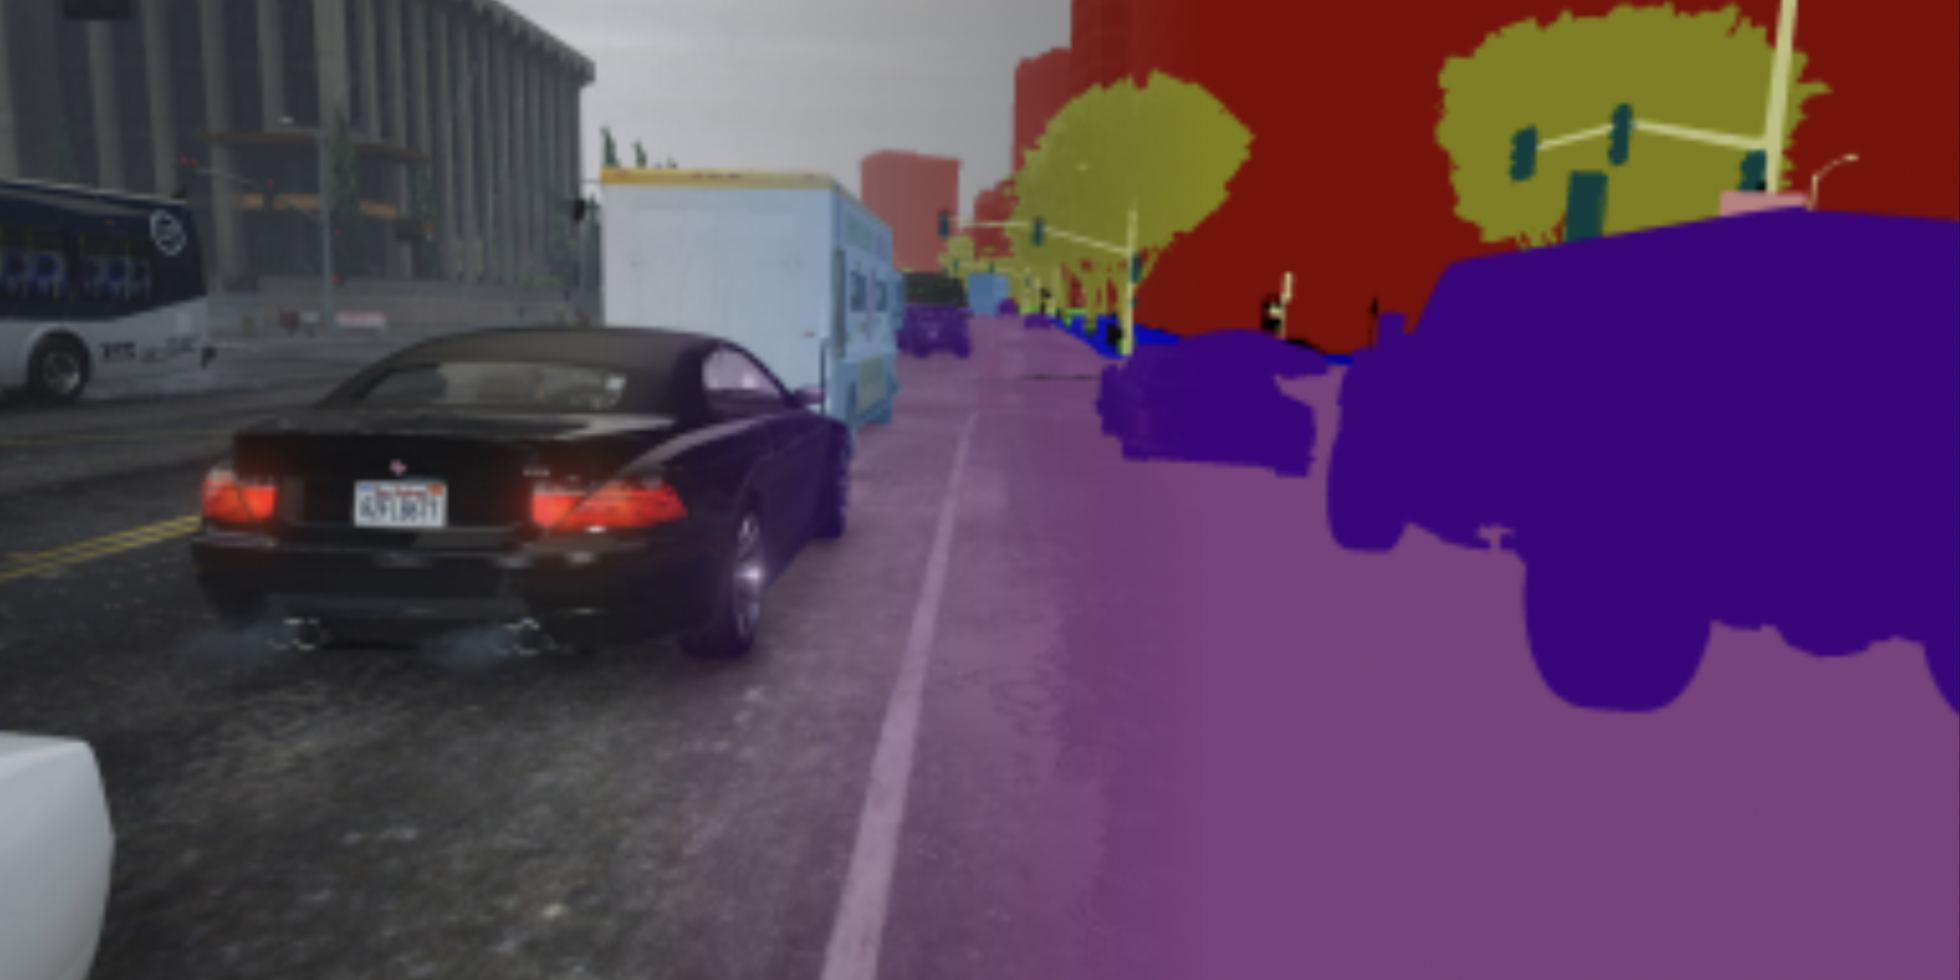
\includegraphics[width=\columnwidth]{img/2-related-work/gtav_semantic_segmentation_overlay_resized.png}
    \caption{GTA Vision \cite{gtav}}
    \label{fig:example-gta}
  \end{subfigure}

  \begin{subfigure}{0.49\columnwidth}
    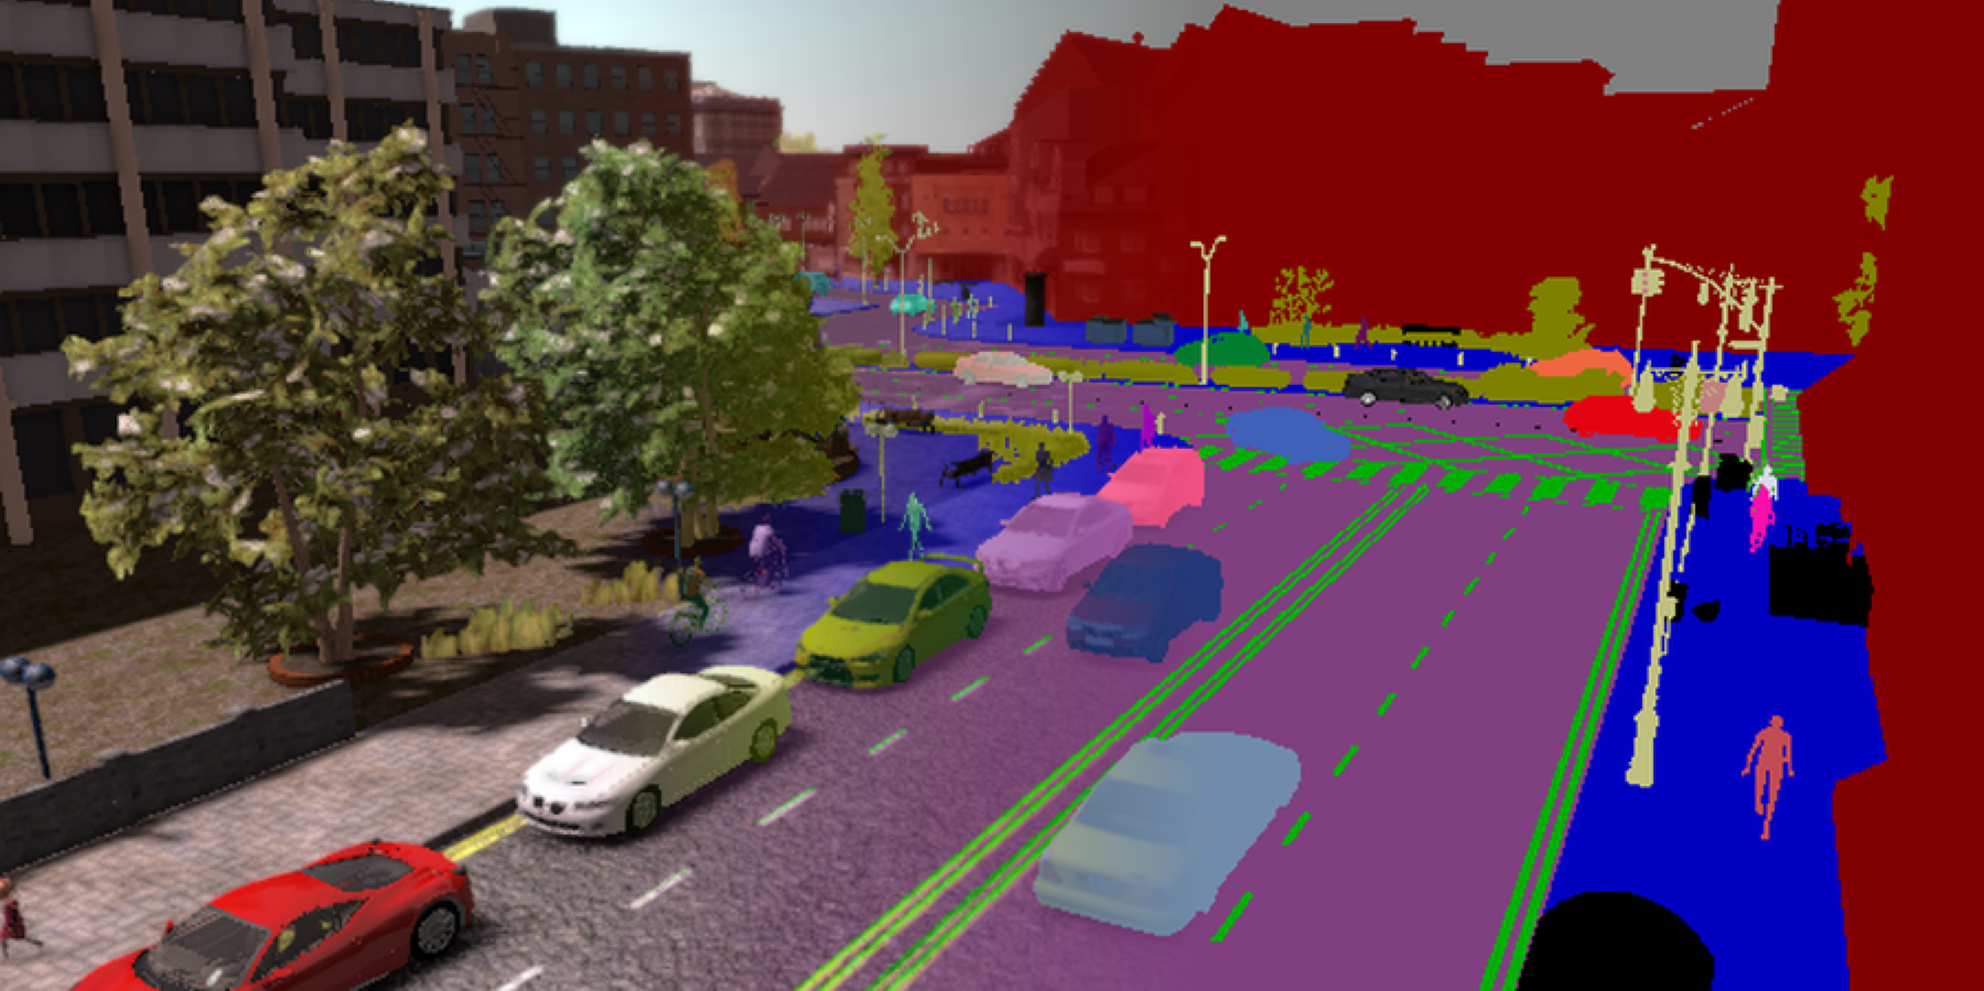
\includegraphics[width=\columnwidth]{img/2-related-work/syntia_semantic_segmentation_overlay.png}
    \caption{SYNTHIA \cite{SYNTHIA}}
    \label{fig:example-syntia}
  \end{subfigure}
  %
  \begin{subfigure}[b]{0.49\columnwidth}
    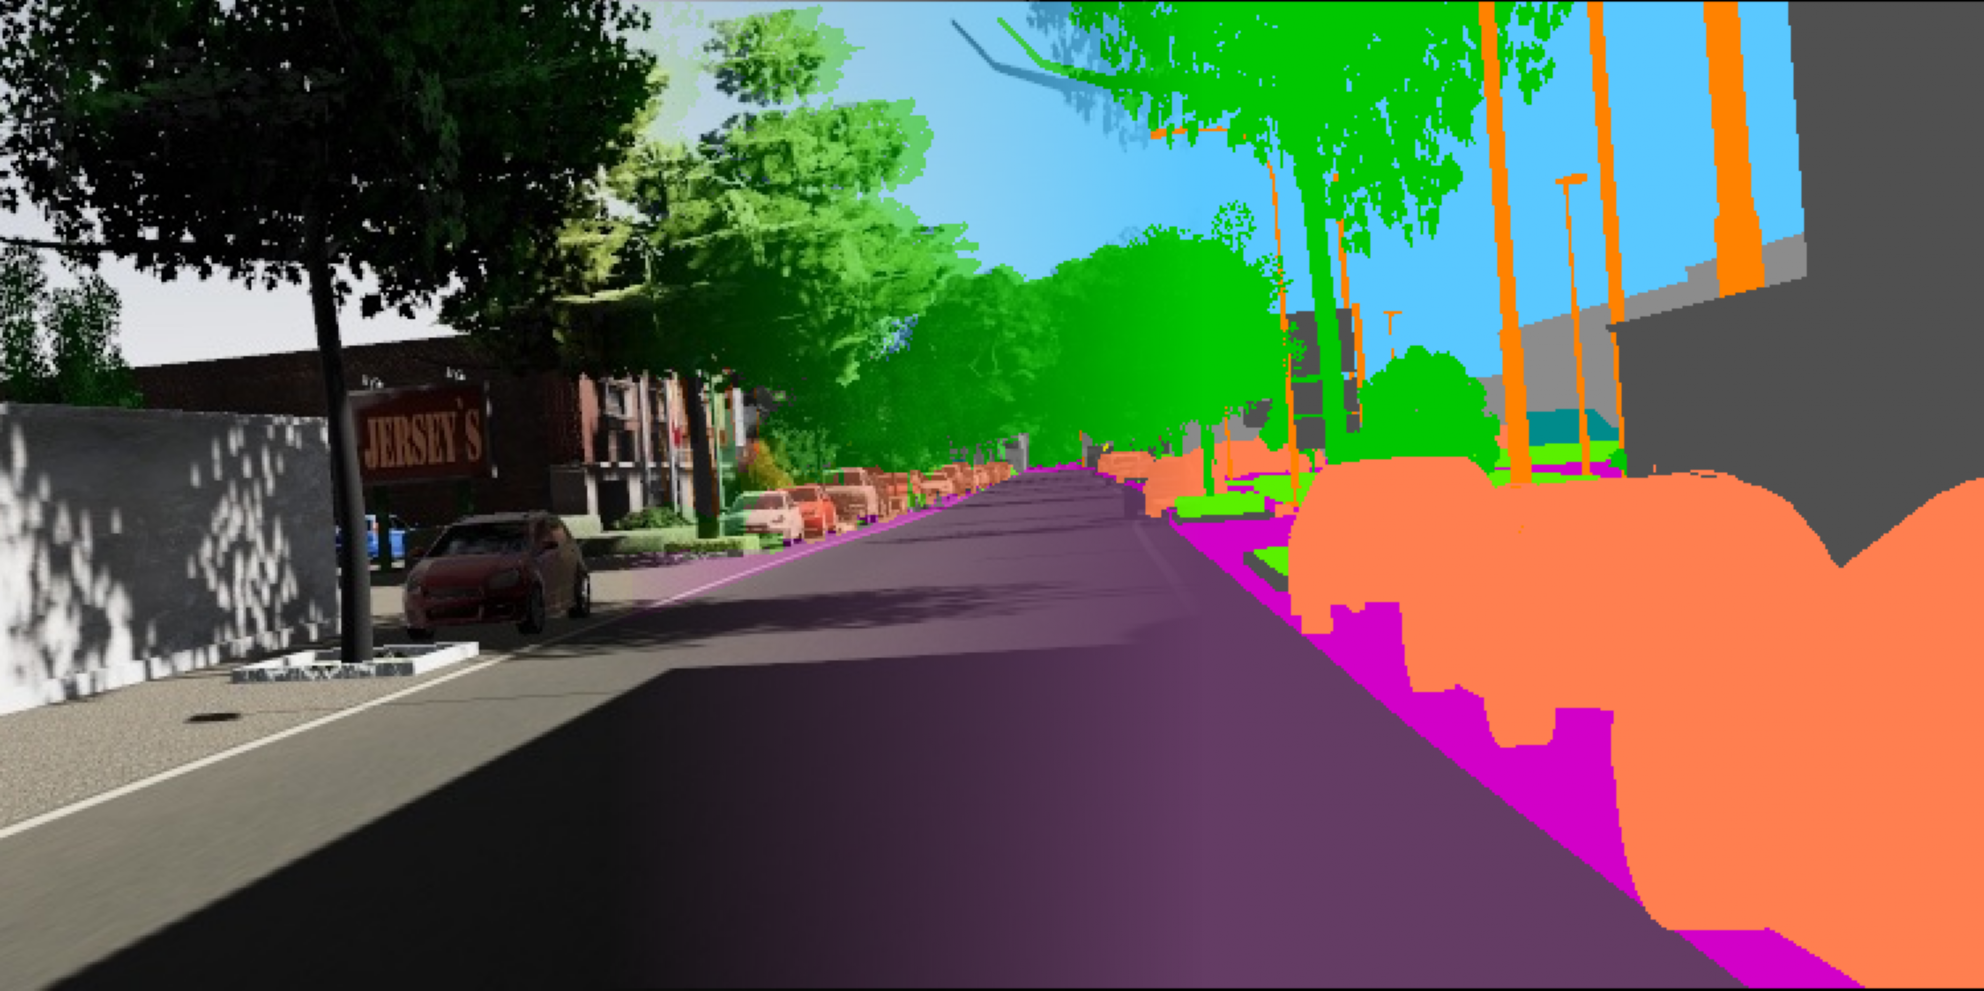
\includegraphics[width=\columnwidth]{img/2-related-work/virtual-kitti_semantic_segmentation_overlay.png}
    \caption {Virtual KITTI \cite{kitty}}
    \label{fig:example-virtual-kitti}
  \end{subfigure}

  \caption[Visual examples of synthetic datasets for urban scenes]{Visual examples of synthetic datasets for urban scenes}
    \label{fig:synthetic-datasets-examples}

\end{figure}

%%%%%%%%%%%%%%%%%%%%%%%%%%%%%%%%%%%%%%%%%%%%%%%%%%%%%%%%%%%%%%%%%%%%%%%%%%%%
%%%%%%%%%%%%%%%%%%%%%%%%%%%  GENERATIVE MODELS   %%%%%%%%%%%%%%%%%%%%%%%%%%%
%%%%%%%%%%%%%%%%%%%%%%%%%%%%%%%%%%%%%%%%%%%%%%%%%%%%%%%%%%%%%%%%%%%%%%%%%%%%

\section{Generative models}
Generative models, particularly those based on neural networks for the generation of new images, have gained significant popularity recently. Unlike discriminative models, which focus on learning the conditional distribution $P(Y|X)$ of output data Y given input data X, generative models aim to learn the joint distribution $P(X,Y)$.

For instance, consider a style transfer problem such as the one proposed in \cite{GUO2020127},  where an image from an urban environment simulator is enhanced to improve its photorealism. A generative model attempts to learn the probability distribution of $(X_i, Y_i)$ pairs, where $X_i$ is an input image and $Y_i$ is an improved version of the image. By sampling an element from the learned distribution of $Y$, a generative model can produce an image that fits within the given domain. Using this approach, generative models can be used to solve tasks such as style transfer, data augmentation, or synthetic data generation.

In contrast, discriminative models concentrate on learning the conditional distribution $P(Y|X)$ to make predictions based on input data $X$. In a classification-like problem, this is done by learning the boundary decision that separates different classes of $Y$ based on the input $X$. For example, in semantic segmentation, a discriminative model predicts the probability of semantic classes based on an input image $X_i$. Although discriminative approaches are very effective for tasks such as classification or regression, they are not suitable for generating new samples by sampling the learned distribution.

In Computer Vision, generative models have advanced significantly due to the availability of large computational resources and datasets with billions of images \cite{schuhmann2022laionb}, which have enabled the training of deep generative models. The design of models with controllable latent spaces has been a key factor in this evolution \cite{Asperti2022}. Latent spaces are low-dimensional representations learned from the input data that capture their underlying structure. By manipulating the values of these latent variables, the generative model can control specific aspects of the output or generate mixtures of output samples \cite{shen2020interpreting}.

Another significant development has been the creation of conditional generative models, which introduce a third element such as a text prompt to guide the generation of samples in a more direct way. This has led to the development of generative models that generate images \cite{rombach2022high, Dalle2}, audio \cite{liu2023audioldm}, or video \cite{ho2022imagen} based on natural language descriptions.

In the following subsections, we review the main architectures that have contributed to the development of generative models and have led to the design of diffusion models\cite{HoEtAl2020}. We pay special attention to the Stable Diffusion architecture \cite{rombach2022high}, which is the focus of this work.


\subsection{Generative architectures}

Deep generative models have achieved impressive results by learning a compact, expressive latent space that enables better synthesis or manipulation of high-dimensional data. However, developing generative architectures has been more challenging than their discriminative counterparts, given the complexity of the task. Nevertheless, machine learning's historical roots in classical architectures like Boltzmann machines \cite{ackley:boltzmann} or autoencoders \cite{rumelhart:errorpropnonote, ballard:modular} provided a foundation for the evolution of these models.

\subsubsection{Autoencoders}

\begin{figure}
    \centering
    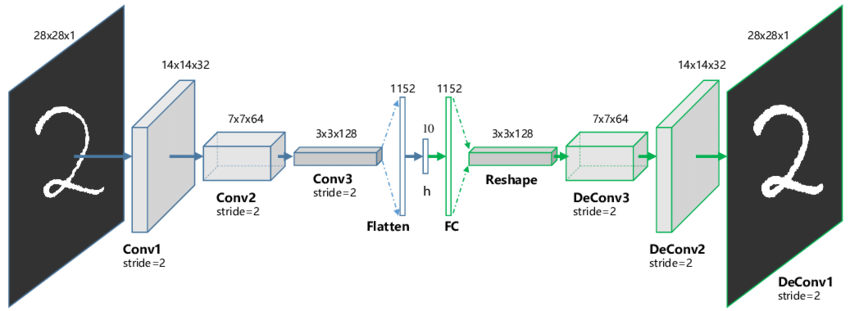
\includegraphics[width=0.8\columnwidth]{img/2-related-work/convolutional-autoencoder.png}
    \caption[Convolutional Autoencoder example]{Convolutional Autoencoder example. Source \cite{neurips/convolutionalautoencoders}.}
    \label{fig:Autoencoder}
\end{figure}


Autoencoders, which date back to the 1980s \cite{rumelhart:errorpropnonote, ballard:modular}, are neural architectures in which a bottleneck layer with a small number of neurons is introduced. In their original design, the network is trained to predict the same output example as the one given as input, but due to the bottleneck layer, a compact representation is forced to be learned. Figure \ref{fig:Autoencoder} shows an example of a Convolutional Autoencoder \cite{neurips/convolutionalautoencoders} following this scheme, which is trained to generate the same digit given as input but with a layer in the middle.

To increase the robustness of the learned representation, researchers have proposed different strategies. For example, Denoising Autoencoders \cite{conf/icml/VincentLBM08} introduce noise in the input samples, Contractive Autoencoders \cite{conf/icml/RifaiVMGB11} include penalty terms, or other works proposed the learning of more complex unsupervised tasks \cite{IEEE/Pathak2016, ieee/zhang2017, Shu_2018_ECCV}.

Autoencoders have been successfully applied to reconstruct noisy images \cite{conf/icml/VincentLBM08} and perform style transfer tasks such as image colorization \cite{zhang2016colorful}. However, when used for generating new synthetic samples using new values of the learned latent space representation in the bottleneck layer, the generated samples may lack variability. Additionally, the learned space may not exhibit desirable properties, as interpolation in the space does not always produce high-quality samples. As a result, other architectures such as Generative Adversarial Networks \cite{NIPS2014_5ca3e9b1} or Latent Diffusion models have become more popular in these types of applications.

\subsubsection{Generative Adversarial Networks (GANs)}

%\begin{figure}
%    \centering
%    \includegraphics[width=0.9\columnwidth]{img/2-related-work/gan-%design.png}
%    \caption[TDiagram of a GAN]{Diagram of a GAN.}
%    \label{fig:gan}
%\end{figure}


%\begin{figure}
%    \centering
%    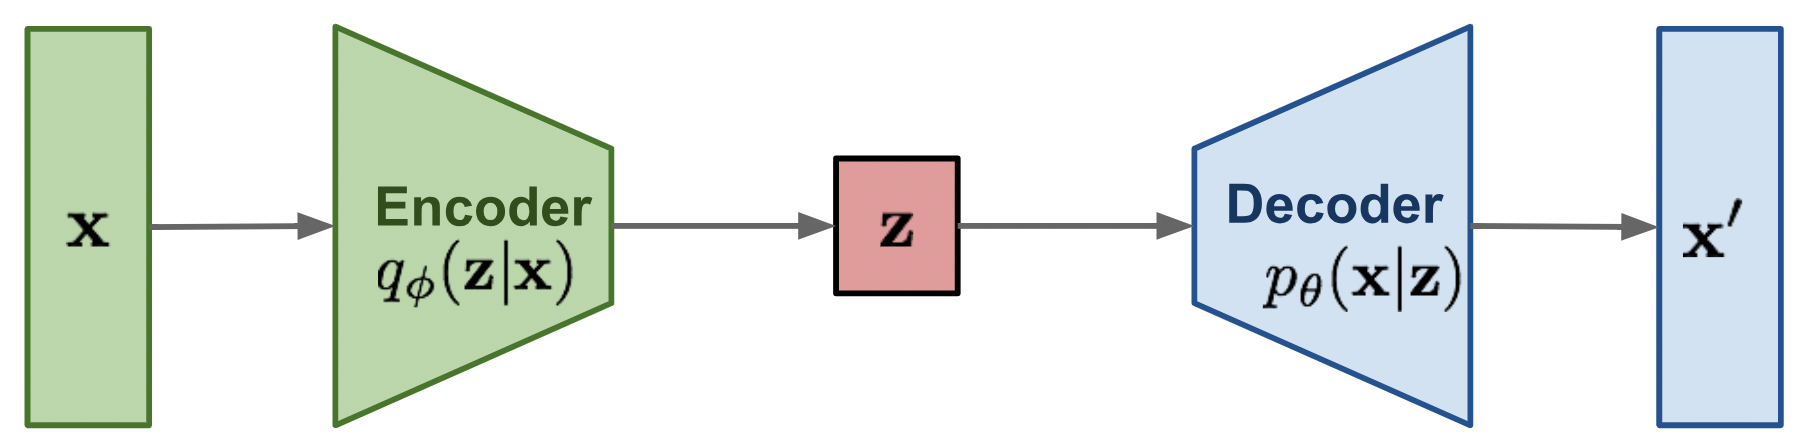
\includegraphics[width=0.9\columnwidth]{img/2-related-work/vae-design.png}
%    \caption[Variational Autoencoder architecture]{Variational Autoencoder architecture \cite{Asperti2021}}
 %   \label{fig:vae}
%\end{figure}

Generative Adversarial Networks (GANs) \cite{NIPS2014_5ca3e9b1} were proposed in 2014 as a revolutionary idea in deep learning, inspiring research in the field ever since. GANs are composed of two neural networks - a generator network $G$ and a discriminator network $D$. The generator network is trained to generate synthetic samples $x'$ from a latent vector $z$ from a known distribution, such as a Gaussian noise distribution. Meanwhile, the discriminator network is trained to classify synthetic and real samples, distinguishing between them. Figure \ref{fig:gan} provides an illustration of this architecture.

The training of GANs is formulated as a search for a Nash equilibrium in a zero-sum game, in which the discriminator seeks to minimize its cost function $J^{(D)}$, while the generator tries to maximize it. The original formulation of $J^{(D)}$ is defined as

\begin{equation}
J^{(D)}(\theta^{(D)}, \theta^{(G)}) = - \frac{1}{2} \mathbb{E}_{x \thicksim X } \log D(x) - \frac{1}{2} \mathbb{E}_{z} \log (1 - D(G(z))).
\end{equation}

However, this theoretical definition is not very practical for training, so variations of the cost functions were proposed to make the training process more stable, but with the same underlying idea \cite{journals/corr/abs-1711-10337}. Even with these modifications, GAN training is dynamic and sensitive to nearly every aspect of its setup, so additional training strategies have been proposed to make them more stable. For example, Progressive GANs \cite{karras2018progressive} have been proposed to improve the stability of GAN training, increasing iteratively the number of layers of the networks during the training epochs. Additionally, strategies to condition generation and gain control in the synthetic samples created have been proposed \cite{radford2015unsupervised, NIPS2016_8a3363ab, conf/nips/ChenCDHSSA16}.


Despite their difficult training process, GANs are one of the most widely used architectures for generative tasks today. One of the reasons for their popularity is the desirable properties of their latent space, which allows for the varied generation of new samples and their control \cite{shen2020interpreting, radford2015unsupervised}. GANs have been successfully applied to a wide range of applications in Computer Vision, including image synthesis \cite{NIPS2016_8a3363ab}, image-to-image translation \cite{Isola2017}, and generation of images from segmentation masks \cite{Wang2018, Park2019}. They have also been applied to video synthesis \cite{wang2018-video} and other applications in natural language processing and signal processing.


\subsubsection{Variational Autoencoders (VAEs)}



\begin{figure}
    \centering
    \begin{subfigure}[b]{0.9\columnwidth}
    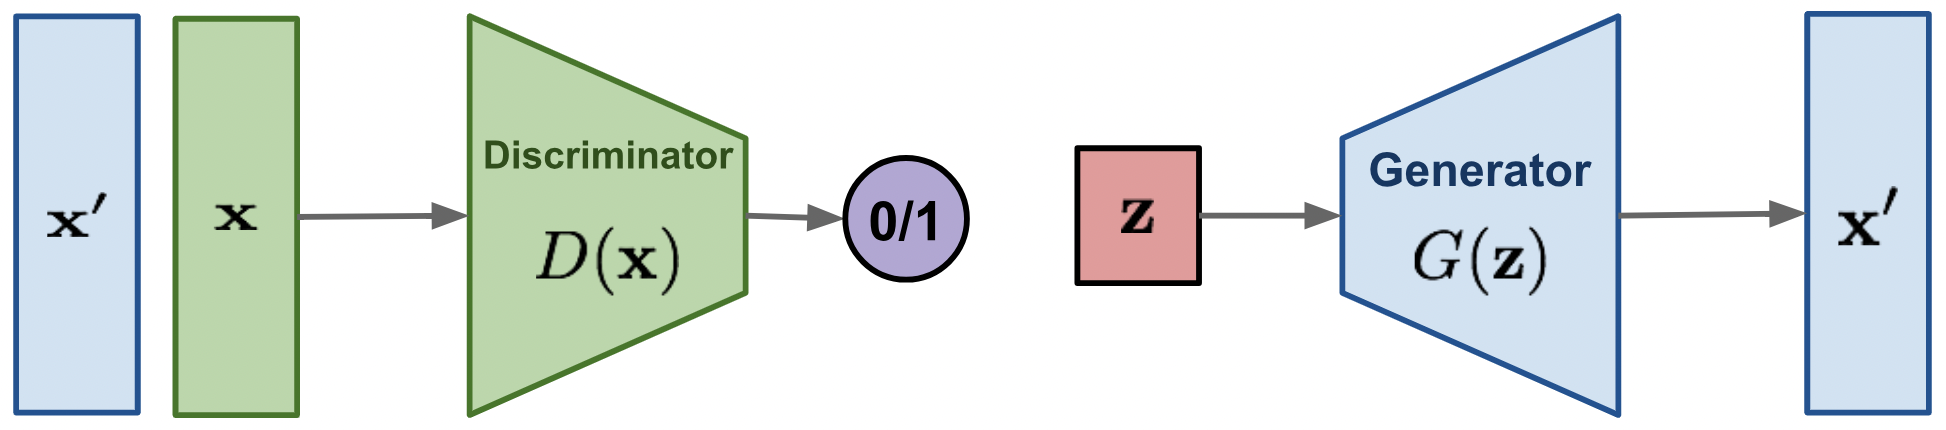
\includegraphics[width=\columnwidth]{img/2-related-work/gan-design.png}
        \caption{GAN Architecture}
        \label{fig:gan}
      \end{subfigure}

  
  \begin{subfigure}[b]{0.9\columnwidth}
    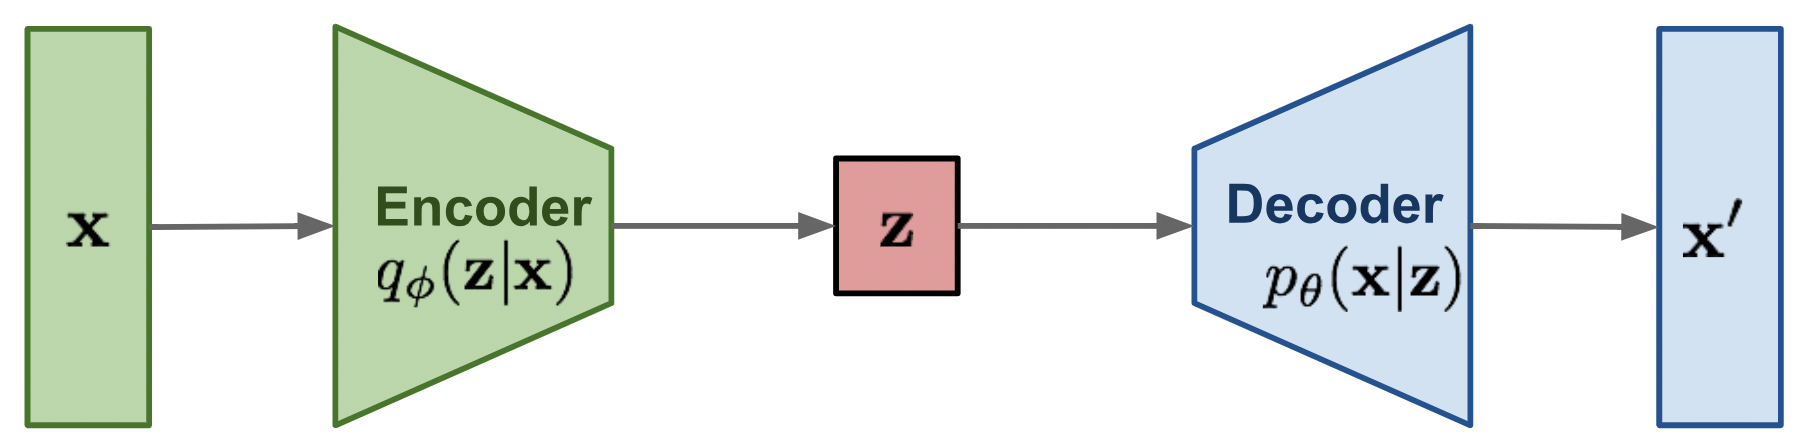
\includegraphics[width=\columnwidth]{img/2-related-work/vae-design.png}
    \caption{VAE Architecture}
    \label{fig:Vae}
  \end{subfigure}
    \caption[VAE and GAN architecture]{VAE and GAN architecture. Source \cite{lilianweng}.}
    \label{fig:gan-vae}
\end{figure}


The Variational Autoencoder (VAE) is a generative model introduced in 2014 \cite{Kingma2014}. Traditional autoencoders can encode input samples into a latent representation in the bottleneck, which can then be used to reconstruct the original input. However, they lack variability in their generated samples, making them less suitable for content generation. The VAE is an extension of traditional autoencoders with a similar encoder-decoder structure, but it adds a probabilistic layer to the encoder. The encoder transforms the input samples into the parameters of a variational distribution, allowing for the generation of new content by sampling from the learned distribution in the latent space. The decoder takes a latent value sampled from the learned distribution and transforms it into the output space.

To train the VAE, the model maximizes the Evidence Lower Bound (ELBO) of the data given the model parameters, which involves computing the reconstruction loss and the Kullback-Leibler divergence between the learned distribution and a prior distribution \cite{Asperti2021}. Thus, the training problem is defined as the maximization of the ELBO, which is formulated as:


\begin{equation}
    L_{\theta, \phi} (x) = \ln p_\phi (x) - D_{KL} (p_\phi(\cdot \, | \, x)\, \| \, q_\theta (\cdot \, | \, x)  )
\end{equation}


The VAE has played an important role in the current revolution of synthetic image generation, with important works such as the VQ-VAE \cite{NIPS2017_7a98af17}, the basis of DALL·E \cite{dalle1}, one of the text-to-image models that preceded the most popular architectures currently employed based on diffusion models \cite{Dalle2, rombach2022high}, in which is also a key component.

\subsection{Diffusion Models}
\label{sec:diffusion-models}

Diffusion Models, specifically Denoising Diffusion Probabilistic Models (DDPMs), are a type of latent generative model proposed in 2020 \cite{HoEtAl2020}. Their main purpose is to generate high-quality samples from a given distribution. DDPMs are based on an iterative process inspired by non-equilibrium thermodynamics, which involves applying a chain of diffusion steps that gradually introduce random noise to the input data. Although diffusion models based on this concept have been proposed before \cite{pmlr-v37-sohl-dickstein15}, the approach of the DDPMs proposed in \cite{HoEtAl2020} enabled the subsequent development of the recently popular text-to-image architectures.


\subsubsection{Fordward diffusion process}

\begin{figure}
    \centering
    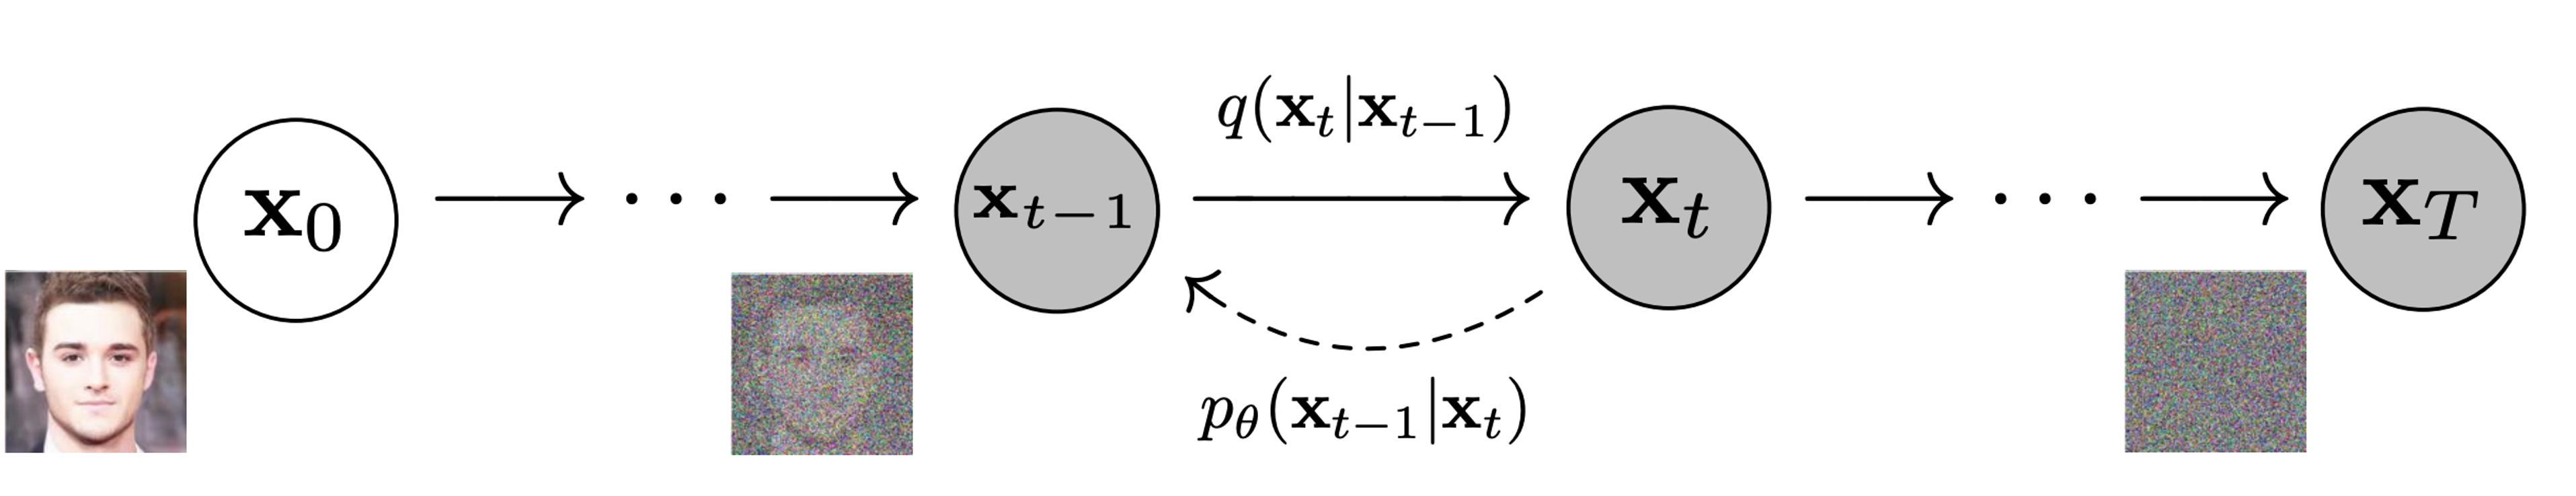
\includegraphics[width=1\columnwidth]{img/2-related-work/fordward-proccess.png}
    \caption[Forward diffusion process of a DDPM]{Forward diffusion process of a DDPM \cite{HoEtAl2020}.}
    \label{fig:fodward-diffusion-process}
\end{figure}

Figure~\ref{fig:fodward-diffusion-process} illustrates the forward diffusion process of a DDPM, in which a data point $\textbf{x}0 \sim q(x)$ from a distribution of input images is gradually transformed through a sequence of $T$ diffusion steps until the image become indistinguishable due to the noise. In its original formulation \cite{HoEtAl2020}, the diffusion process uses Gaussian noise with a predefined variance schedule $\{\beta_t \in (0, 1)\}_{t=1}^T$. When $T \rightarrow \infty$, the result of the process, $\textbf{x}_T$, is distributed as an isotropic Gaussian variable. With this formulation, for an arbitrary timestep $t$, the process $q$ is distributed as


\begin{equation}
    q(\textbf{x}_t |\textbf{x}_{t-1}) \sim \mathcal{N}\left(\sqrt{1 - \beta_t}\textbf{x}_{t-1}, \beta_t \textbf{I}\right).
\end{equation}

Employing a cumulative product of the timestep variances $\Tilde{\alpha}_t = 1 - \prod_{i=1}^t (1 - \beta_t)$, the distribution can be reparameterized in terms of the original input $\textbf{x}_0$ as


\begin{equation}
    q(\textbf{x}_t |\textbf{x}_{t-1}) \sim \mathcal{N}\left(\sqrt{1 - \Tilde{\alpha}_t}\textbf{x}_0,  \Tilde{\alpha}_t \textbf{I}\right).
\end{equation}

\subsubsection{Reverse diffusion process}
 
If we could reverse the diffusion process and sample from $q(x_{t-1}|x_t)$, we could reconstruct the original sample from a noise input $\textbf{x}_T$. However, this inverse process is intractable, thus it is not possible to estimate it directly. Instead, we can train a model $p_\theta$ to approximately perform the inverse process using the Algorithm \ref{alg:training} described in \cite{HoEtAl2020}, in which the function $\epsilon_{\theta}$ learns to predict the noise $\epsilon$ added in a timestep from $\textbf{x}_t$.


\begin{multicols}{2}

\begin{algorithm}[H]
\caption{DDPM training}\label{alg:training}
\begin{algorithmic}
\Repeat
\State $\textbf{x}_0 \sim q(\textbf{x}_0)$
\State $t \sim \text{Uniform}(\{1, \ldots, T\})$
\State $\textbf{$\epsilon$} \sim \mathcal{N}(\textbf{0}, \textbf{I})$
\State Take gradient descent step on
\State \footnotesize{$\hspace{2em}  \nabla_\theta\left\| \textbf{$\epsilon$} - \textbf{$\epsilon$}_{\theta} \left(\sqrt{1 - \Tilde{\alpha}_t}\textbf{x}_0 + \sqrt{ \Tilde{\alpha}_t}\textbf{$\epsilon$}, \,t\right) \right\|^2$ }\normalsize{}
\Until converged
\end{algorithmic}
\end{algorithm}


\begin{algorithm}[H]
\caption{DDPM sampling}\label{alg:sampling}
\begin{algorithmic}
\State
\vspace{0.7em}
\State $\textbf{x}_T \sim \mathcal{N}(\textbf{0}, \textbf{I})$ 
\For{$t=T, \ldots , 1$}
\State $\textbf{z} \sim \mathcal{N}(\textbf{0}, \textbf{I})$ if $t>1$, else $\textbf{z}=\textbf{0}$
\State $\textbf{x}_{t-1} =$ \scriptsize{$\frac{1}{\sqrt{1 - \beta_t}} \left( \textbf{x}_t  - \frac{\beta_t}{\sqrt{ \Tilde{\alpha}_t}} \textbf{$\epsilon$}_\theta(\textbf{x}_t, t)   \right) + \sqrt{\beta_t} \textbf{z}$} \normalsize{}
\EndFor
\State \Return $x_0$
\end{algorithmic}
\end{algorithm}
\end{multicols}


The training algorithm, samples an initial data point $x_0$ from the input distribution $q(x_0)$ and a random timestep $t$ between 1 and $T$. Then, it samples a random vector \textbf{$\epsilon$} from the noise distribution. It takes a gradient descent step on the difference between \textbf{$\epsilon$} and $\textbf{$\epsilon$}_{\theta}$, evaluated at $(\sqrt{1 - \Tilde{\alpha}_t}\textbf{x}_0+\sqrt{\Tilde{\alpha}_t}\textbf{$\epsilon$}_t, t)$. The sampling process (Algorithm \ref{alg:sampling}), generates a sample $\textbf{x}_T$ from the noise distribution and performs a reverse diffusion process over $T$ timesteps using $\epsilon_\theta$ to obtain the reconstructed image.

In practice, several variations of the original proposal have been developed to address specific challenges and use cases. For instance, there have been introduced mechanisms for conditional generation \cite{Dhariwal2021} and the use of text as input \cite{Dalle2, rombach2022high}. In addition, other classes of noises, schedules, and losses are employed to improve the convergence of the inverse process modeling the noise as an ODE \cite{song2021scorebased}. However, diffusion-based models that have recently gained popularity, such as DALLE·2 \cite{Dalle2} or Stable Diffusion \cite{rombach2022high}, are based on the same underlying idea as above.

\subsubsection{Stable Diffusion}


Stable Diffusion \cite{rombach2022high} is a widely used latent diffusion model for image generation. Its open-source nature has allowed for the emergence of many research works exploring the architecture and a wide range of applications. The model has gained significant traction since its launch, thanks to the release of several pre-trained versions. In this work, we focus on the Stable Diffusion 2.0 version\footnote{Stable Diffusion 2.0: \href{https://huggingface.co/stabilityai/stable-diffusion-2}{huggingface.co/stabilityai/stable-diffusion-2} (Accessed June 2023).}, a 1.1 billion parameters version pre-trained on the LAION 5-billion image dataset \cite{schuhmann2022laionb}. The architecture is highly versatile, with variations that allow it to perform image manipulation tasks such as image inpainting, outpainting, and super-resolution. However, in this work we focus on the original text-to-image sampling mode.

The architecture comprises three main components: a deep language model to generate word embeddings, a VAE that encodes and decodes latent vectors into images, and a time-conditional denoising network responsible for denoising the latent models in the diffusion process. Additionally, some versions of the model include a final classifier to filter out Not Safe for Work (NSFW) content. A diagram illustrating the components of the model can be seen in Figure \ref{fig:stable-diffusion}.

The deep language model $\tau_{\theta}$, generally a CLIP model \cite{Radford2021LearningTV}, is responsible for transforming the input text prompts in natural language into word embeddings. These embeddings are vectors of fixed size in a more appropriate space in which there are preserved structures that maintain semantic relationships between words. These vectors are then used in the diffusion process to condition the generation by guiding the generated images by means of attention mechanisms. Generally, this language component is pre-trained separately and its weights are not modified during the training of the diffusion model \cite{dosovitskiy2020vit}.

The conditional denoiser network $\epsilon_{\theta}$, generally a conditional U-NET as in Stable Diffusion 2, is in charge of performing the iterative process of inverse diffusion. Unlike the original U-NET \cite{UNET} (see Figure~\ref{fig:unet}), a variation is used in which cross-attention layers are introduced, in charge of introducing the information of the text embeddings to guide the denoising process. Later, in Section \ref{sec:explainability-dm}, we dwell on these attention mechanisms, since we extract from them the information of the semantic segmentation masks during the generation of synthetic images.

The VAE \cite{Kingma2014} is formed by an encoder $\mathcal{E}$ and a decoder $\mathcal{D}$ (see Figure \ref{fig:Vae}). The encoder $\mathcal{E}$ is in charge of transforming images to the latent space of the network where the diffusion process is applied. Although the encoder is mainly used for training the architecture, it can be used in the sampling process to initialize the diffusion process with an image. The VAE decoder $\mathcal{D}$ transforms the U-NET output after applying the inverse diffusion process to convert the denoised latent variable $z$ into an image.

\begin{figure}
    \centering
    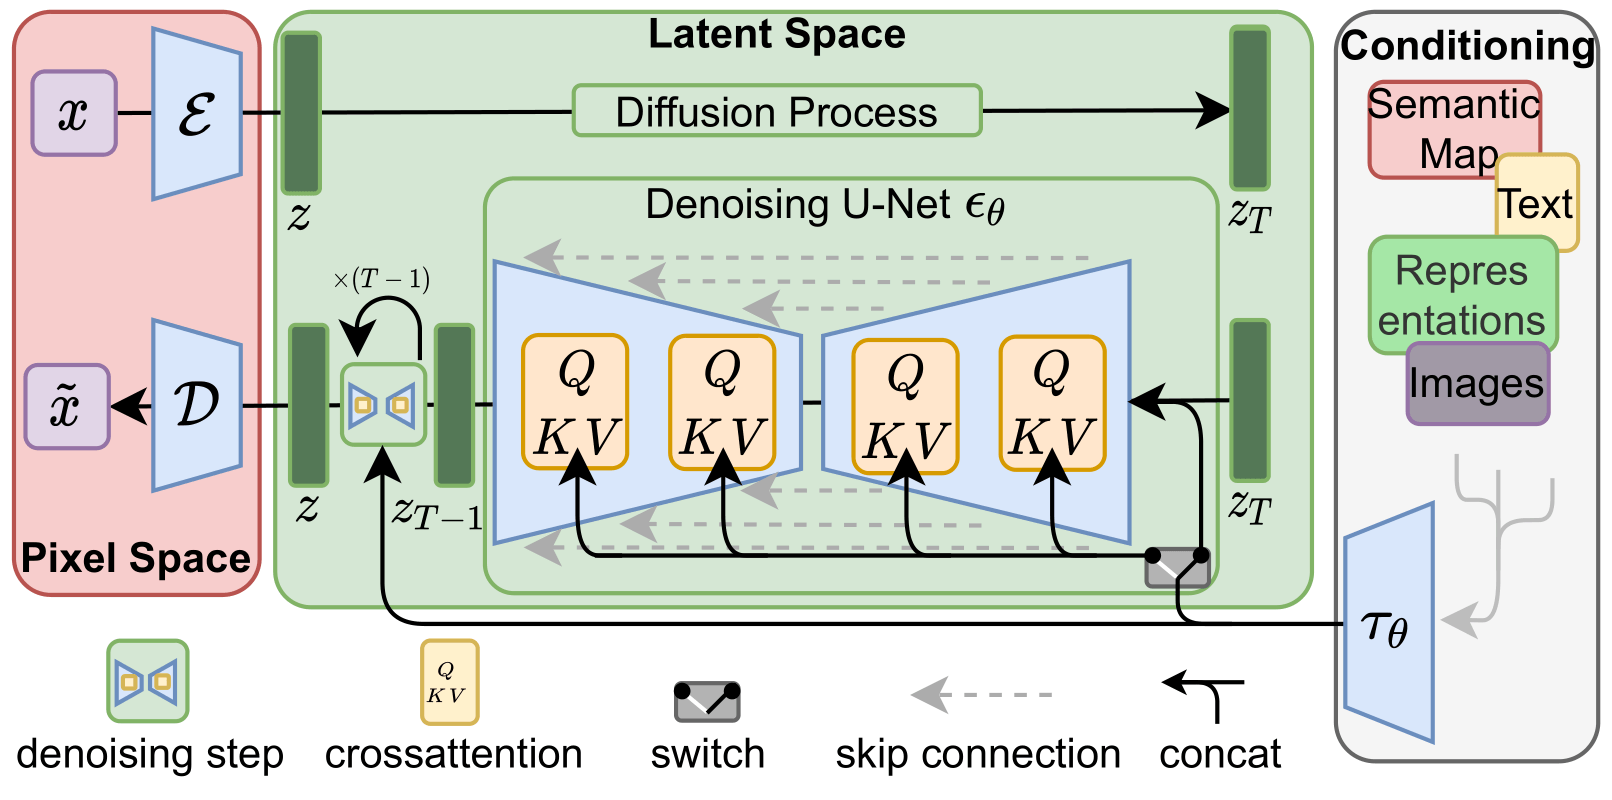
\includegraphics[width=\columnwidth]{img/2-related-work/stable-diffusion-architecture.png}
    \caption[Stable Diffusion architecture]{Stable Diffusion architecture. Source \cite{rombach2022high}.}
    \label{fig:stable-diffusion}
\end{figure}


\subsubsection{Challenges in Synthetic Data Generation using Stable Diffusion}
%Nota: En esta sección añadiré los diferentes avances que aparezcan en SD. Como text-to-video, reinforcement learning, text-to-audio, cambio de losses, etc... Como varia semana a semana lo cambiaré al final con lo que haya resultado más trascendente en los próximos meses.

Despite the progress made in text-to-image generation, there are still several challenges that need to be addressed. One major challenge is the difficulty of generating images that accurately match the input text. This is particularly challenging when dealing with too specific concepts or complex scenes that require a high level of visual understanding.

Several methods have been proposed to address this challenge, including the use of additional constraints on the architecture to respect a predefined structure, such as a given segmentation map, during image generation \cite{zhang2023adding}. Other works focus on adjusting the attention generated on the cross-attention layers during image generation to mitigate the model from discarding part of the text information given as input \cite{AttendAndExcite}.

Improving the accuracy of text prompts is also an important issue that has been addressed in recent works. The term \emph{prompt engineering} has become popular to describe the optimization of queries to improve image generation \cite{promptEngineering}. Among the lines of research focused on automating this process, we can highlight works focused on obtaining queries that generate images as similar as possible to a given image \cite{HardPromptsMadeEasy} or the use of reinforcement learning to train systems capable of generating better text prompts \cite{Promptist}. These methods can significantly improve the generation of high-quality images from text without modifying the text-to-image architecture.

All these challenges motivate the development of methods for the explainability of latent diffusion image generation. A better understanding of the underlying processes allows for the creation of text prompts that are better suited to generate images, as well as the development of more sophisticated techniques to interact with these models. 
These topics are explored in more detail in Section \ref{sec:explainability}.


%%%%%%%%%%%%%%%%%%%%%%%%%%%%%%%%%%%%%%%%%%%%%%%%%%%%%%%%%%%%%%%%%%%%%%%%%%%%
%%%%%%%%%%%%%%%%%%%%%%%%%%%%%  EXPLAINABILITY   %%%%%%%%%%%%%%%%%%%%%%%%%%%%
%%%%%%%%%%%%%%%%%%%%%%%%%%%%%%%%%%%%%%%%%%%%%%%%%%%%%%%%%%%%%%%%%%%%%%%%%%%%

\section{Explainability}
\label{sec:explainability}

The rise of Deep Learning has paved the way for remarkable advances in Computer Vision, enabling us to solve tasks that would have been difficult to tackle in the past \cite{Chai2021}. However, the increasing complexity of these models and their widespread use across various domains have brought new challenges. One such challenge is the lack of transparency and interpretability in these models, which can hinder their potential applications in real-world scenarios.

Traditionally, these models have been treated as a black box, with little attention paid to their internal workings. However, this approach presents significant limitations, as it becomes difficult to explain how the model arrived at a particular decision. Furthermore, the lack of transparency in these models poses legal and ethical risks, as accountability becomes challenging when the decision-making process is not transparent \cite{Gerlings2020ReviewingTN}.

To address these issues, the field of explainable Artificial Intelligence (\emph{XAI}) has emerged, aiming to develop methods that make these models more transparent and interpretable \cite{SALEEM2022165}. This is particularly relevant in Computer Vision \cite{QuanshiZHANG}, where interpretability and explainability can be fundamental for understanding the inner workings of models and addressing issues such as bias and fairness \cite{Kirill2022}.


While the terms explainability and interpretability are often used interchangeably due to their close relation, they are distinct tasks. Interpretability measures the extent to which a model can associate a cause with an effect, based on its input and output variables. For instance, \emph{Shapley values} can be used to assign a numeric weight to each input variable, reflecting its influence on an output prediction \cite{shapley}. On the other hand, explainability is a broader task that pertains to the ability of a model's decisions to be understood by humans, including the ability to describe the model's behavior and the factors that influence it \cite{Gerlings2020ReviewingTN}. For example, an explanation of a model's behavior might involve identifying specific features in an input image that caused the model to produce a particular output prediction \cite{extremalPerturbations}. Alternatively, it could entail identifying which features activate a certain layer or node of a neural network, providing insights into the hierarchy of features used by the network \cite{optimizationInput}, and identifying potential biases in the model.

In this section, we explore the issue of explainability in Computer Vision, focusing specifically on diffusion models. We begin by reviewing the concept of explainability in Computer Vision and the main methods currently employed. Next, we delve into the specific challenges related to the explainability of diffusion models, discussing recent developments and identifying potential avenues for future research. Finally, we discuss the relevance of explainability in the scenario of synthetic image generation for semantic segmentation, highlighting the significance of transparent and interpretable models in real-world applications.

\subsection{Explainability in Computer Vision}

\begin{figure}
\centering
 \begin{subfigure}{0.3\columnwidth}
    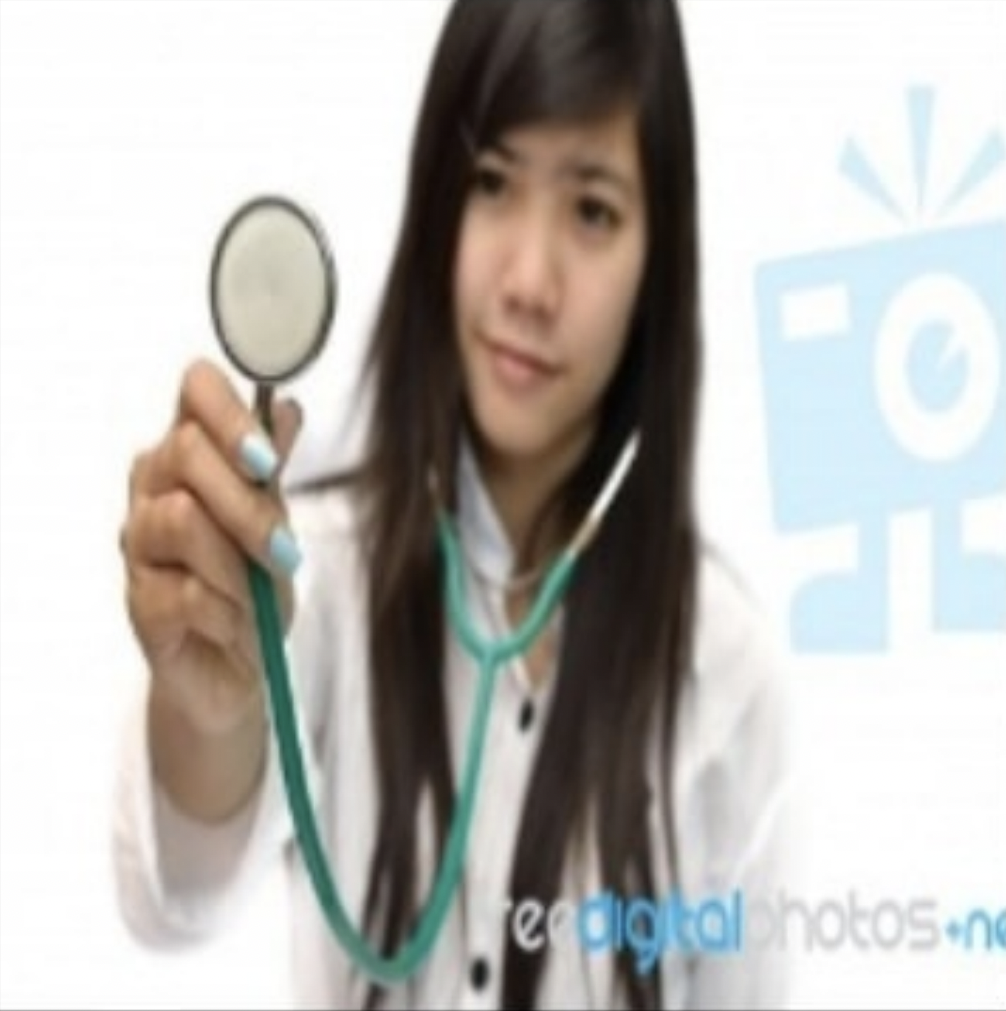
\includegraphics[width=0.95\columnwidth, height=0.95\columnwidth]{img/2-related-work/bias-computer-vision-doctor.png}
    \caption{Original}
    \label{fig:biased-model-cam-image}
  \end{subfigure}
  \begin{subfigure}{0.3\columnwidth}
    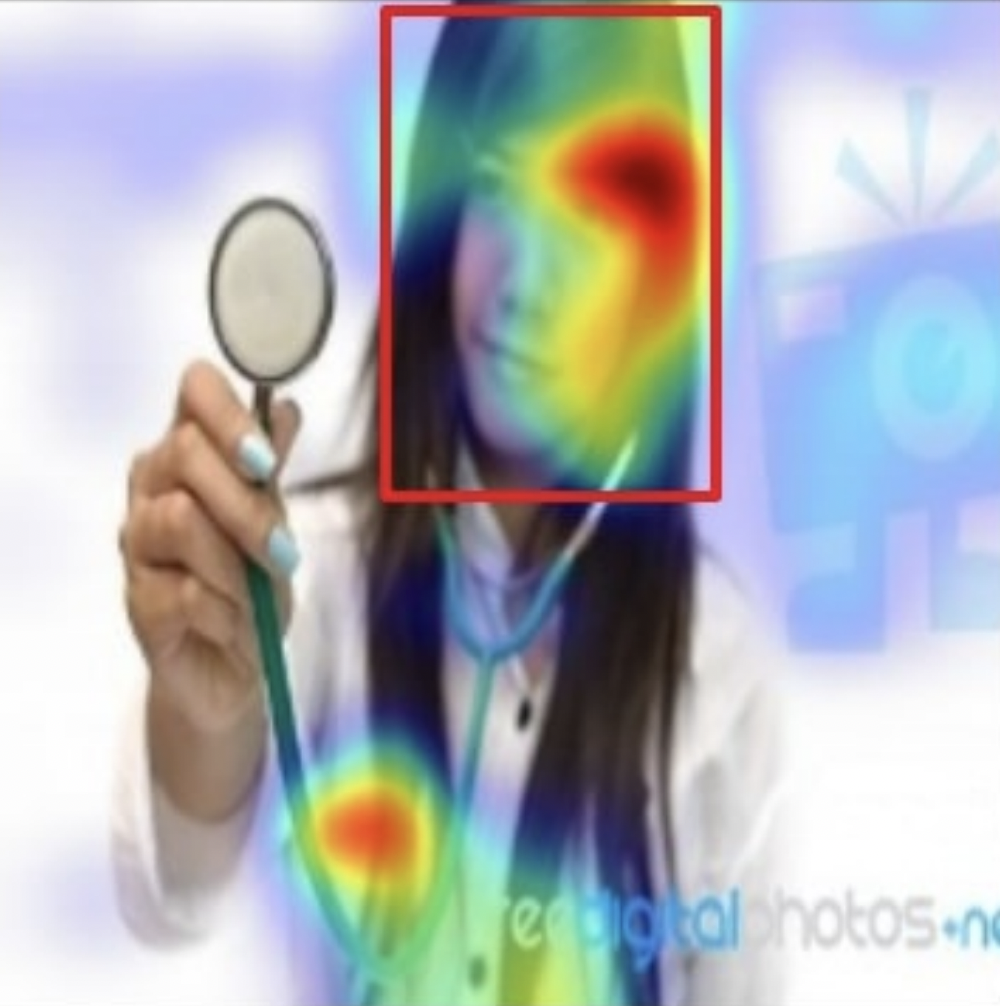
\includegraphics[width=0.95\columnwidth, height=0.95\columnwidth]{img/2-related-work/bias-computer-vision-doctor-nurse.png}
    \caption{CAM of ``Nurse''}
    \label{fig:biased-model-cam-nurse}
  \end{subfigure}
  \begin{subfigure}{0.3\columnwidth}
    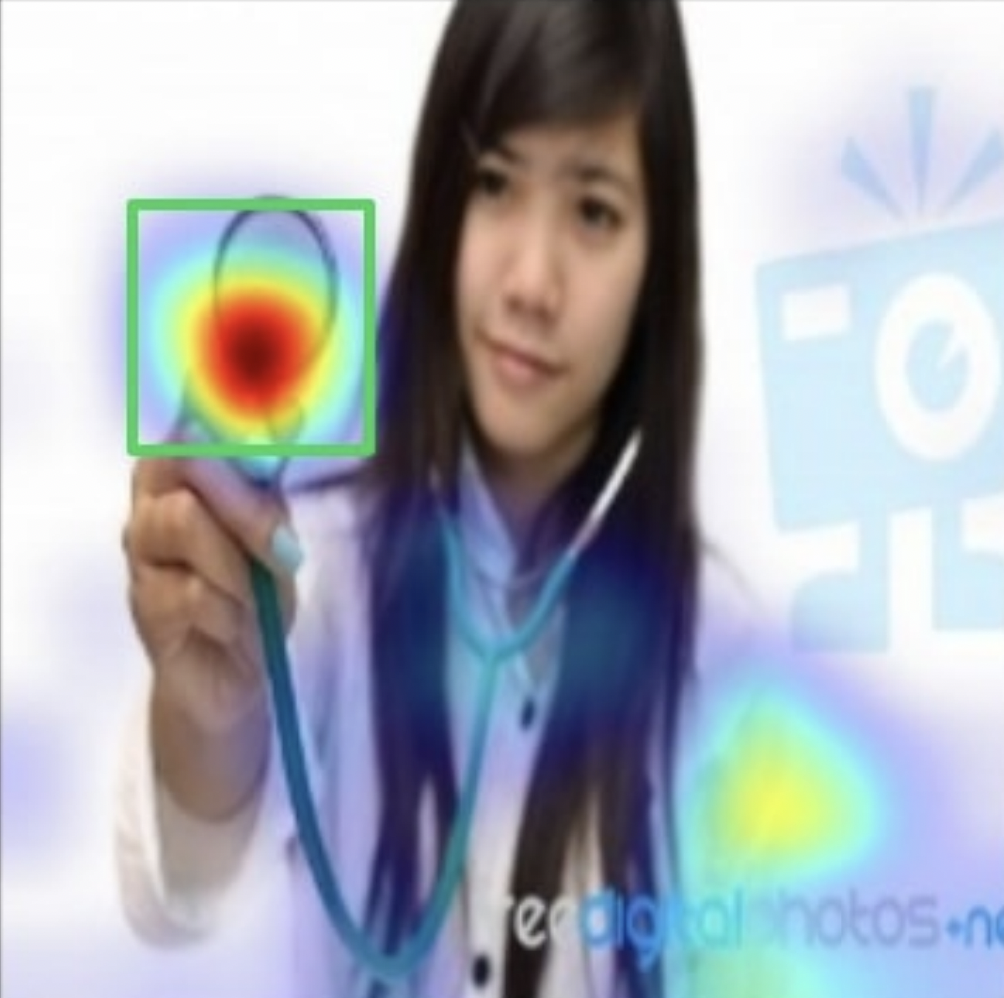
\includegraphics[width=0.95\columnwidth, height=0.95\columnwidth]{img/2-related-work/bias-computer-vision-doctor-cam.png}
    \caption{CAM of  ``Doctor''}
    \label{fig:biased-model-doctor}
  \end{subfigure}

  \caption[Class activation maps (Grad-CAM) of a biased model]{Class activation map (Grad-CAM) of a biased model. (a) A stock photo image labeled as ``Doctor''. (b) Areas on which a biased model relies to predict the ``Nurse'' class (c) and ``Doctor''. Source \cite{gradcam}.}
  \label{fig:realbiased-model}
\end{figure}


\begin{figure}
\centering
 \begin{subfigure}{0.3\columnwidth}
    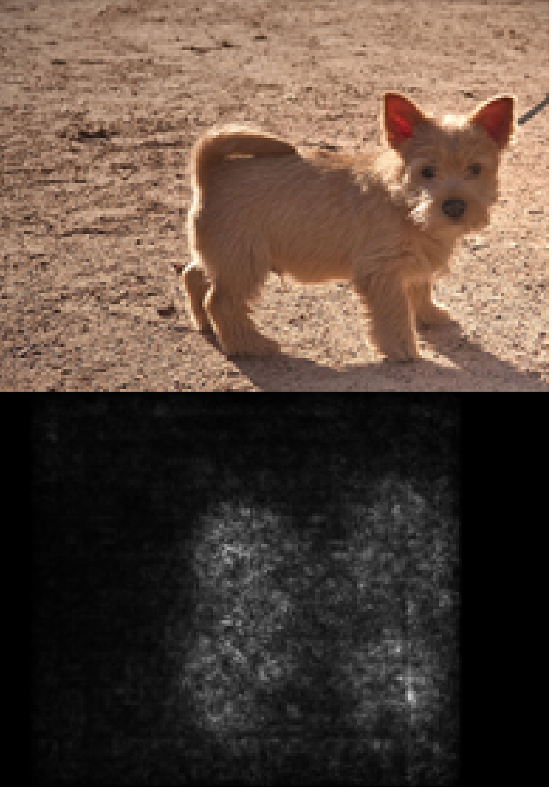
\includegraphics[width=0.95\columnwidth]{img/2-related-work/dog-saliency-map.png}
   %\caption{Saliency map \cite{Simonyan2013DeepIC}}
   \caption{}
    \label{fig:example-interpretability-1}
  \end{subfigure}
  \begin{subfigure}{0.3\columnwidth}
    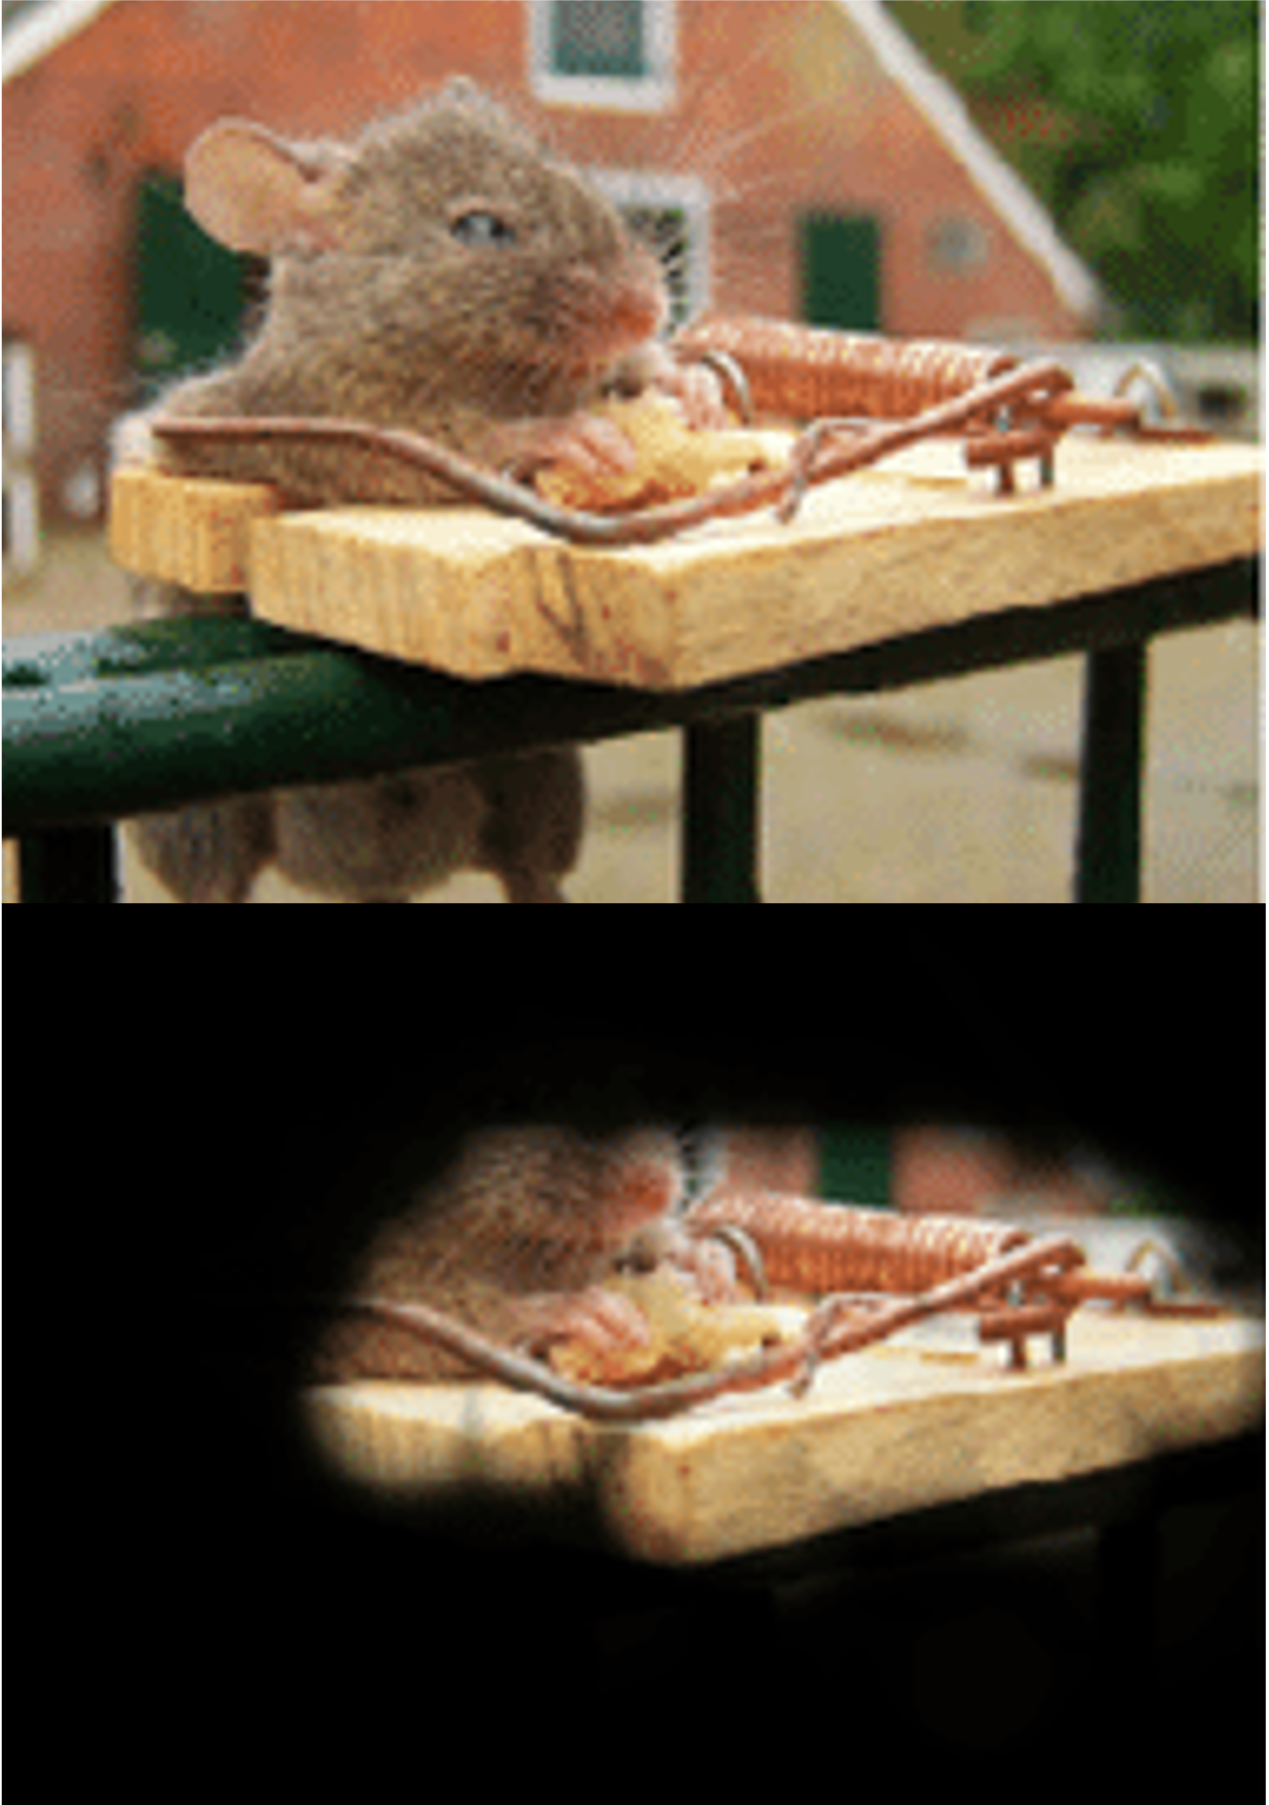
\includegraphics[width=0.95\columnwidth]{img/2-related-work/mouse-extremal-perturbations.png}
    %\caption{Extremal Perturbation \cite{Fong2019}}
    \caption{}
    \label{fig:example-interpretability-2}
  \end{subfigure}
  \begin{subfigure}{0.3\columnwidth}
    \includegraphics[width=0.95\columnwidth]{img/2-related-work/inceptionism.png}
    %\caption{Inception }
    \caption{}
    \label{fig:example-interpretability-3}
  \end{subfigure}
  \caption[Examples of explainability methods for Computer Vision]{Examples of explainability methods for Computer Vision. (a) Image of a dog and the corresponding Saliency Map \cite{Simonyan2013DeepIC} of the class ``Dog''. (b) Image of a mouse in a trap and a masked version using Extremal perturbations \cite{Fong2019} with the most discriminative part to classify the image as ``mouse trap''. (c) Feature optimization to maximize a convolutional layer response \cite{Mordvintsev2015InceptionismGD} using an image of a savanna as prior. The processed image contains more highlighted edges, indicating that the layer is activated in the presence of this type of low-level feature. Source \cite{Simonyan2013DeepIC, Fong2019, Mordvintsev2015InceptionismGD}.}
  \label{fig:example-interpretability}
  \end{figure}

Explainability methods for Computer Vision are becoming increasingly important due to regulatory requirements and the need for increased reliability \cite{Gerlings2020ReviewingTN}. Computer vision models are particularly susceptible to acquiring biases present in the datasets on which they are trained \cite{Kirill2022, GeirhosRMBWB19}. Figure \ref{fig:realbiased-model} provides a striking example of this phenomenon, where an image labeled as ``Doctor'' (\ref{fig:biased-model-cam-image}) is accompanied by the regions on which a biased model relies to classify the image as "Nurse" (\ref{fig:biased-model-cam-nurse}) and ``Doctor'' (\ref{fig:biased-model-doctor}), both sex-agnostic classes \cite{gradcam}. Notably, the biased model places a disproportionate weight on the long hair region to classify the image as ``Nurse'', and on the stethoscope to classify it as ''Doctor``. Such biases can result in harmful outcomes in various scenarios and may adversely impact the model's performance. However, explainability methods can help to detect and mitigate the impact of these biases.

To achieve explainability in Computer Vision, researchers use established methods to interpret convolutional models. These methods can be classified into three main approaches: gradient-based attribution methods, perturbation-based methods, and techniques for feature visualization using optimization techniques.

Gradient-based attribution methods are commonly used in Computer Vision to determine the contribution of each input feature to the final model prediction through the backpropagation of gradients. One such method is saliency maps \cite{Simonyan2013DeepIC}, which calculate the gradient of a class score with respect to the input image, highlighting the aspects that most influence the image's classification as that class (Figure \ref{fig:example-interpretability-1}). Other popular methods, such as Class Activation Maps (CAM) \cite{CAM} and Gradient-weighted Class Activation Mapping (GradCAM) \cite{gradcam}, use global average pooling in conjunction with gradient backpropagation to create class activation maps. These maps are heatmaps that identify the most relevant areas for classifying an image, as illustrated in Figure \ref{fig:realbiased-model}. These attribution maps can be used to detect potential biases in classification models and can even be used to perform object location and semantic segmentation of the object being classified.

Perturbation-based methods involve masking or altering input features to observe the effect on the model output. Examples of perturbation-based methods are Minimal Image Representation \cite{Zhou2014ObjectDE} and Extremal Perturbations \cite{Fong2019}, which attempt to learn a mask that removes parts of an image that have minimal impact on the output of a model, as illustrated in Figure \ref{fig:example-interpretability-2}. In contrast, other methods, such as Meaningful Perturbations \cite{Fong2017InterpretableEO}, try to blur or mask the parts of an image that most influence the model prediction.

Feature visualization methods are focused on understanding the behavior of neural networks by finding inputs that activate certain parts of the network through optimization. One commonly used technique is activation maximization, which involves maximizing the activation of a saliency map \cite{Simonyan2013DeepIC}. However, to make the obtained inputs more interpretable, additional methods like Feature Inversion \cite{featureInversion} or Inceptionism \cite{Mordvintsev2015InceptionismGD} utilize images as priors to generate more meaningful representations. By optimizing an input image that amplifies the activation of specific neurons in a neural network, we can obtain images that highlight the features that those neurons are encoding. This enables us to gain insights into whether a layer is filtering a specific texture or a semantic concept, as shown in Figure \ref{fig:example-interpretability-3}.

Explainability research in Computer Vision is currently a highly active field, with new techniques used in other domains still being explored, such as the use of counterfactual explanations \cite{conterfactual2019}, adversarial attacks \cite{Ghorbani_Abid_Zou_2019}, or causal reasoning \cite{Liu2022CausalRM}. While current methods have shown promise in detecting and mitigating biases in Computer Vision models, their application still poses several challenges. For example, there is a lack of consistency across techniques, which makes it difficult to compare and evaluate their interpretations. Measuring the effectiveness of these methods in practice is also complicated, especially when considering their impact on downstream tasks. Additionally, most established techniques are based on image classification, and extending them into generative tasks is still an emerging issue.

In recent years, explainability research has extended to other domains, such as natural language processing, where models such as transformers have been shown to achieve state-of-the-art performance on a variety of tasks but can be difficult to interpret \cite{attentionisnot,clark-etal-2019-bert}. One approach to interpretability in language models is to use attention mechanisms to visualize the words or phrases that the model is focusing on during prediction \cite{attentionisnot}. 

Overall, explainability methods are critical in ensuring the reliability and trustworthiness of machine learning models. As machine learning continues to be deployed in increasingly complex and sensitive applications, the development of effective and practical explainability methods will be essential for achieving transparency and accountability.


\subsection{Explainability of Diffusion Models}
\label{sec:explainability-dm}

The emergence of diffusion models for image generation is a relatively recent development, and research on methods for their explainability is still an emerging topic. Current research in this area focuses on text-attribution methods, which attempt to answer the question of which parts of an image are influenced most by each word in the text prompt. These methods aim to create heat maps of the influence of each word in the input text on the resulting image.

Unfortunately, early investigations in this direction found that methods based on gradients and perturbations cannot be adapted to diffusion models due to the iterative process involved in the diffusion process. Gradient methods require a backpropagation pass for every pixel for all $T$ time steps, which makes computation intractable and the process highly unstable. Perturbation-based methods result in significantly different images even with minor perturbations, making them unsuitable for diffusion models \cite{DAAM}.

As a result, the main methods being developed for explainability in diffusion models are based on ideas from natural language processing, where attention to words indicates lexical attribution \cite{clark-etal-2019-bert}. These methods exploit the conditional mechanisms based on cross-attention, where the text guides the image generation. One such method is the Diffusion Attentive Attribution Maps (DAAMs) \cite{DAAM}, whose maps are based on these attention mechanisms.

Other methods being explored for explainability in diffusion models involve modifying the attention process to highlight the attention of the tokens that need to be explained \cite{AttendAndExcite}, or by perturbing the attention \cite{deb2023atman}.

However, since this is still an emerging topic, many aspects remain to be investigated, and there are many potential issues that may expand the applications of these methods. In this work, we focus on exploring DAAMs for the extraction of semantic segmentation masks during synthetic image generation. As the DAAM method is important for our work, we provide a more detailed explanation of the process in Chapter \ref{cha:methodology}.




% https://github.com/heejkoo/Awesome-Diffusion-Models#inverse-problem